% ============================================================================
%  Doc W -- SPEAR3 RF Station Wiring and Interconnection Reference
%  Build:  powershell -ExecutionPolicy Bypass -File build.ps1 -Doc W
%          (runs scripts/docw-gen.js first, which writes generated/ from data/)
%  Engine: LuaLaTeX (required -- see the Unicode note in preamble.tex)
% ============================================================================
\documentclass[letterpaper,11pt]{article}
% ============================================================================
%  SPEAR3 RF System documentation -- shared preamble
%  Engine: LuaLaTeX.  Build with build.ps1 (latexmk -lualatex).
% ============================================================================

\usepackage[letterpaper,top=1in,bottom=1in,left=1.05in,right=1.05in]{geometry}

% --- fonts -----------------------------------------------------------------
\usepackage{fontspec}
\setmainfont{TeX Gyre Termes}
\setsansfont{TeX Gyre Heros}
\setmonofont{Consolas}[Scale=0.86]

% --- Unicode safety --------------------------------------------------------
% LuaLaTeX DROPS unmapped glyphs SILENTLY -- an unmapped U+03BC turns "8 uF"
% into "8 F".  Every non-ASCII character used in these documents is mapped
% here.  The build script fails if the log reports "Missing character".
\usepackage{newunicodechar}
\newunicodechar{μ}{\ensuremath{\mu}}      \newunicodechar{µ}{\ensuremath{\mu}}
\newunicodechar{Ω}{\ensuremath{\Omega}}   \newunicodechar{≈}{\ensuremath{\approx}}
\newunicodechar{≥}{\ensuremath{\geq}}     \newunicodechar{≤}{\ensuremath{\leq}}
\newunicodechar{≠}{\ensuremath{\neq}}     \newunicodechar{×}{\ensuremath{\times}}
\newunicodechar{÷}{\ensuremath{\div}}     \newunicodechar{±}{\ensuremath{\pm}}
\newunicodechar{−}{\ensuremath{-}}        \newunicodechar{√}{\ensuremath{\sqrt{}}}
\newunicodechar{α}{\ensuremath{\alpha}}   \newunicodechar{β}{\ensuremath{\beta}}
\newunicodechar{φ}{\ensuremath{\varphi}}  \newunicodechar{ω}{\ensuremath{\omega}}
\newunicodechar{Δ}{\ensuremath{\Delta}}   \newunicodechar{τ}{\ensuremath{\tau}}
\newunicodechar{θ}{\ensuremath{\theta}}   \newunicodechar{λ}{\ensuremath{\lambda}}
\newunicodechar{π}{\ensuremath{\pi}}      \newunicodechar{σ}{\ensuremath{\sigma}}
\newunicodechar{₀}{\ensuremath{_0}}       \newunicodechar{₁}{\ensuremath{_1}}
\newunicodechar{₂}{\ensuremath{_2}}       \newunicodechar{²}{\ensuremath{^2}}
\newunicodechar{³}{\ensuremath{^3}}       \newunicodechar{⁴}{\ensuremath{^4}}
\newunicodechar{⁻}{\ensuremath{^-}}       \newunicodechar{⁺}{\ensuremath{^+}}
\newunicodechar{→}{\ensuremath{\rightarrow}}
\newunicodechar{←}{\ensuremath{\leftarrow}}
\newunicodechar{↔}{\ensuremath{\leftrightarrow}}
\newunicodechar{⇒}{\ensuremath{\Rightarrow}}
\newunicodechar{⊕}{\ensuremath{\oplus}}   \newunicodechar{∥}{\ensuremath{\parallel}}
\newunicodechar{°}{\ensuremath{^\circ}}   \newunicodechar{·}{\ensuremath{\cdot}}
\newunicodechar{≪}{\ensuremath{\ll}}      \newunicodechar{≫}{\ensuremath{\gg}}
\newunicodechar{✓}{\checkmark}            \newunicodechar{⚠}{\textbf{!}}
\newunicodechar{–}{--}                    \newunicodechar{—}{---}

% --- maths and units -------------------------------------------------------
\usepackage{amsmath,amssymb}
\usepackage{siunitx}
\DeclareSIUnit\voltampere{VA}
\DeclareSIUnit\VAR{var}
% range-phrase must not rely on literal spaces (LaTeX strips them from a key
% value, so "{ to }" renders as "10to20") and must force text mode (siunitx
% sets numbers in math, where a bare "--" becomes two minus signs).
\sisetup{per-mode=symbol,range-phrase={\text{--}},range-units=single,
         group-minimum-digits=4,detect-weight=true}

% --- tables ----------------------------------------------------------------
\usepackage{longtable,booktabs,array,tabularx,multirow}
\usepackage{ragged2e}
\setlength{\LTleft}{0pt}\setlength{\LTright}{0pt}
\renewcommand{\arraystretch}{1.18}
% left-aligned, hyphenating paragraph column used by every wide table
\newcolumntype{P}[1]{>{\RaggedRight\arraybackslash}p{#1}}
% Same, but \small: for dense tables.  The size must live in the column type --
% wrapping a longtable in {\small ...} breaks its page-breaking \write.
\newcolumntype{Q}[1]{>{\small\RaggedRight\arraybackslash}p{#1}}

% --- graphics and figures --------------------------------------------------
\usepackage{graphicx}
% Resolved from the document's own folder, which is the working directory.
\graphicspath{{../common/}{../common/photos/}{../common/generated/}}
\usepackage{float}
\usepackage[font=small,labelfont=bf,width=0.92\linewidth]{caption}
\usepackage{comment}
% longtable* (from ltcaption, loaded by caption) is for tables without a caption,
% but longtable still steps the table counter.  Give it a private anchor and take
% the number back, so the numbered tables run 1, 2, 3 and their links are unique.
\makeatletter
\AddToHook{env/longtable*/begin}{\def\theHtable{nocap.\arabic{LT@tables}}}
\AddToHook{env/longtable*/after}{\addtocounter{table}{-1}}
\makeatother

% A figure must not drift out of the section it belongs to.  With 47 floats
% LaTeX will otherwise push them pages away from the text that discusses them.
\usepackage[section]{placeins}

% Default float parameters are tuned for papers with two or three figures.
% This document is figure-dense, so allow more of a page to be float and more
% floats per page; without this, figures queue up and drift several pages.
\renewcommand{\topfraction}{0.88}
\renewcommand{\bottomfraction}{0.70}
\renewcommand{\textfraction}{0.10}
\renewcommand{\floatpagefraction}{0.72}
\setcounter{topnumber}{3}
\setcounter{bottomnumber}{2}
\setcounter{totalnumber}{5}

% Image size policy.  Photographs are capped in BOTH width and height so that
% no figure can ever exceed roughly half a page, whatever its aspect ratio.
\newlength{\photomaxh}\setlength{\photomaxh}{0.34\textheight} % ~1/3 page
\newlength{\widemaxh} \setlength{\widemaxh}{0.46\textheight}  % ~1/2 page

% \photofig{file}{caption}{label}      -- default, about 1/3 page
\newcommand{\photofig}[3]{%
  \begin{figure}[htbp]\centering
    \includegraphics[width=0.62\linewidth,height=\photomaxh,keepaspectratio]{#1}%
    \caption{#2}\label{#3}
  \end{figure}}
% \widefig{file}{caption}{label}       -- for detailed schematics, about 1/2 page
\newcommand{\widefig}[3]{%
  \begin{figure}[htbp]\centering
    \includegraphics[width=0.94\linewidth,height=\widemaxh,keepaspectratio]{#1}%
    \caption{#2}\label{#3}
  \end{figure}}
% \smallfig{file}{caption}{label}      -- for low-resolution sources
\newcommand{\smallfig}[3]{%
  \begin{figure}[htbp]\centering
    \includegraphics[width=0.44\linewidth,height=0.26\textheight,keepaspectratio]{#1}%
    \caption{#2}\label{#3}
  \end{figure}}
% \tallfig{file}{caption}{label}       -- portrait-orientation photographs.
% A tall photo capped at \photomaxh comes out only ~45 mm wide, so these are
% capped by height instead and allowed a narrower column.
\newcommand{\tallfig}[3]{%
  \begin{figure}[tbp]\centering
    \includegraphics[width=0.46\linewidth,height=0.4\textheight,keepaspectratio]{#1}%
    \caption{#2}\label{#3}
  \end{figure}}
% two portrait photographs side by side under one caption:
% \tallpairfig{fileA}{subA}{labA}{fileB}{subB}{labB}{caption}{label}
\newcommand{\tallpairfig}[8]{%
  \begin{figure}[tbp]\centering
    \begin{minipage}[b]{0.46\linewidth}\centering
      \includegraphics[width=\linewidth,height=0.40\textheight,keepaspectratio]{#1}%
      \subcaption{#2}\label{#3}
    \end{minipage}\hfill
    \begin{minipage}[b]{0.46\linewidth}\centering
      \includegraphics[width=\linewidth,height=0.40\textheight,keepaspectratio]{#4}%
      \subcaption{#5}\label{#6}
    \end{minipage}
    \caption{#7}\label{#8}
  \end{figure}}
% two photographs side by side, each about 1/4 page
\newcommand{\pairfig}[6]{%
  \begin{figure}[htbp]\centering
    \begin{minipage}[t]{0.48\linewidth}\centering
      \includegraphics[width=\linewidth,height=0.26\textheight,keepaspectratio]{#1}%
      \subcaption{#2}\label{#3}
    \end{minipage}\hfill
    \begin{minipage}[t]{0.48\linewidth}\centering
      \includegraphics[width=\linewidth,height=0.26\textheight,keepaspectratio]{#4}%
      \subcaption{#5}\label{#6}
    \end{minipage}
  \end{figure}}
\usepackage{subcaption}

% --- diagrams --------------------------------------------------------------
\usepackage{tikz}
\usetikzlibrary{arrows.meta,positioning,fit,backgrounds,calc,shapes.geometric,
                shapes.misc,chains,decorations.pathreplacing,patterns,matrix}
\usepackage{pgfplots}\pgfplotsset{compat=1.18}
\usepackage{rotating}                  % sidewaysfigure, if a portrait page is wanted
\usepackage{pdflscape}                 % landscape: rotates the PAGE in the PDF
\usepackage[export]{adjustbox}         % max width= / max height= on a box

% Shrink a diagram to the text width only if it would otherwise overflow, so
% figures drawn at their natural scale are never enlarged or needlessly shrunk.
\newsavebox{\fitbox}
\newenvironment{fitpicture}
  {\begin{lrbox}{\fitbox}}
  {\end{lrbox}%
   \ifdim\wd\fitbox>\linewidth
     \resizebox{\linewidth}{!}{\usebox{\fitbox}}%
   \else
     \usebox{\fitbox}%
   \fi}

% House diagram style.  Keep every block diagram in these styles so the
% document reads as one drawing set rather than a scrapbook.
\definecolor{cCtrl}{HTML}{1F4E79}   % control / EPICS
\definecolor{cPlc} {HTML}{7F6000}   % PLC / interlock
\definecolor{cPwr} {HTML}{843C0C}   % high power
\definecolor{cRf}  {HTML}{2E6B34}   % RF signal path
\definecolor{cNeut}{HTML}{3B3B3B}
\tikzset{
  blk/.style   ={draw=cNeut,fill=white,rounded corners=1.6pt,align=center,
                 inner sep=4pt,font=\scriptsize,minimum height=8mm},
  ctrl/.style  ={blk,draw=cCtrl,fill=cCtrl!7,text=cCtrl!85!black},
  plc/.style   ={blk,draw=cPlc, fill=cPlc!8, text=cPlc!80!black},
  pwr/.style   ={blk,draw=cPwr, fill=cPwr!7, text=cPwr!85!black},
  rf/.style    ={blk,draw=cRf,  fill=cRf!7,  text=cRf!80!black},
  grp/.style   ={draw=black!35,dashed,rounded corners=3pt,inner sep=7pt},
  lbl/.style   ={font=\scriptsize\itshape,text=black!62},
  sig/.style   ={-{Stealth[length=2.2mm]},draw=cNeut,thick},
  fib/.style   ={sig,densely dashed},
  bus/.style   ={draw=cNeut,line width=1.1pt},
  tag/.style   ={font=\tiny,inner sep=1.4pt,fill=white,text=black!70},
}
% consistent caption for a TikZ figure
\newcommand{\diagcap}[2]{\caption{#1}\label{#2}}

% --- lists, misc -----------------------------------------------------------
\usepackage{enumitem}
\setlist{nosep,leftmargin=1.35em}
\providecommand{\tightlist}{%   emitted by pandoc for compact lists
  \setlength{\itemsep}{0pt}\setlength{\parskip}{0pt}}
\usepackage[table]{xcolor}
\usepackage{soul}
\usepackage{microtype}
\usepackage{fancyhdr}
\usepackage{lastpage}
\usepackage{needspace}

% --- callout box for warnings / key findings -------------------------------
\usepackage[most]{tcolorbox}
\newtcolorbox{keynote}[1][]{colback=black!3,colframe=black!45,boxrule=0.4pt,
  arc=1.5pt,left=5pt,right=5pt,top=4pt,bottom=4pt,fontupper=\small,#1}
\newtcolorbox{warnbox}[1][]{colback=cPwr!5,colframe=cPwr!70,boxrule=0.7pt,
  arc=1.5pt,left=5pt,right=5pt,top=4pt,bottom=4pt,fontupper=\small,#1}

% --- cross references and links --------------------------------------------
\usepackage[hyphens]{url}
\usepackage[hidelinks,pdfusetitle,bookmarksnumbered]{hyperref}
\usepackage[capitalise,nameinlink]{cleveref}
\crefname{section}{\S}{\S\S}
\Crefname{section}{Section}{Sections}
% Spell out "Figure" for \cref too; cleveref's default abbreviates it to "Fig.",
% which reads inconsistently beside \Cref in the same sentence.
\crefname{figure}{Figure}{Figures}
% Lowercase \cref on a section prints "§5.7" / "§§10.2--10.5" -- no space after
% the sign and an en-dash range, matching the hand-written style it replaced.
\crefformat{section}{\S#2#1#3}
\crefrangeformat{section}{\S\S#3#1#4--#5#2#6}
\crefmultiformat{section}{\S#2#1#3}{ and~\S#2#1#3}{, \S#2#1#3}{ and~\S#2#1#3}

% Repository paths are long and unhyphenatable; allow breaks after / and .
% Long file paths and CamelCase document names have no natural break points, so
% url's default break set is not enough: allow a break before any capital and
% after the usual separators.
\newcommand{\fpath}[1]{{\ttfamily\small\Urlmuskip=0mu plus 1mu\relax
  \def\UrlBreaks{\do\/\do\.\do\-\do\_\do\:\do\A\do\B\do\C\do\D\do\E\do\F\do\G
    \do\H\do\I\do\J\do\K\do\L\do\M\do\N\do\O\do\P\do\Q\do\R\do\S\do\T\do\U
    \do\V\do\W\do\X\do\Y\do\Z}%
  \urlstyle{tt}\nolinkurl{#1}}}
\setlength{\emergencystretch}{2em}

% --- headers ---------------------------------------------------------------
\pagestyle{fancy}\fancyhf{}
\renewcommand{\headrulewidth}{0.3pt}
\fancyhead[L]{\footnotesize\nouppercase{\rightmark}}
\fancyhead[R]{\footnotesize\thepage\ / \pageref{LastPage}}
\renewcommand{\sectionmark}[1]{\markright{\thesection\quad #1}}
\fancypagestyle{plain}{\fancyhf{}\renewcommand{\headrulewidth}{0pt}%
  \fancyfoot[C]{\footnotesize\thepage}}

\setcounter{tocdepth}{2}
\setcounter{secnumdepth}{3}


% Column width for longtables with @{} edges: fraction of \linewidth minus the
% per-column share of the inter-column padding, 2(n-1)/n \tabcolsep.
\newcommand{\cw}[2]{\dimexpr #1\linewidth-#2\tabcolsep\relax}
% Dense data tables: footnote size, ragged right; \uchyph=0 keeps signal names
% such as HEARTBEAT from being hyphenated.
\newcolumntype{F}[1]{>{\footnotesize\RaggedRight\uchyph=0\arraybackslash}p{#1}}
% A repository path at table size: no letter-spacing, breaks only at separators.
\newcommand{\dpath}[1]{{\ttfamily\scriptsize\Urlmuskip=0mu\relax
  \def\UrlBreaks{\do\/\do\.\do\-\do\_}\urlstyle{tt}\nolinkurl{#1}}}

% Counts written by the generator (\WDrawings, \WVerified, ...).
% generated by scripts/docw-gen.js from data/ -- do not edit
\newcommand{\WDrawings}{103}
\newcommand{\WVerified}{45}
\newcommand{\WWithErrata}{21}
\newcommand{\WNotRead}{0}
\newcommand{\WRead}{0}
\newcommand{\WPEPII}{18}
\newcommand{\WCited}{0}
\newcommand{\WReference}{19}
\newcommand{\WUntitled}{0}
\newcommand{\WErrata}{22}
\newcommand{\WErrataOpen}{5}
\newcommand{\WChecks}{24}
\newcommand{\WChecksOpen}{23}
\newcommand{\WConnections}{135}
\newcommand{\WPLCModules}{20}
\newcommand{\WPLCPoints}{272}
\newcommand{\WStatusList}{45 verified against other sources, 20 with errata, 1 disputed, 19 reference documents with no wiring to check and 18 drawn or written for PEP-II}


\hypersetup{pdftitle={SPEAR3 RF Station Wiring and Interconnection Reference},
  pdfauthor={Faya Wang},pdfsubject={Doc W R0 - Draft for review}}

\title{\vspace{-1.4cm}\bfseries SPEAR3 RF Station\\[2mm]
       \Large Wiring and Interconnection Reference}
\author{}
\date{}

\begin{document}
\maketitle
\thispagestyle{plain}

\begin{center}
\begin{minipage}{0.86\linewidth}\small
\begin{tabular}{@{}ll@{}}
\textbf{Document ID}    & Doc W \\
\textbf{Revision}       & R0 \\
\textbf{Status}         & Draft \\
\textbf{Author}         & Faya Wang \\
\textbf{Reviewer}       & Jim Sebek \\
\textbf{Classification} & Tier 2 --- Station reference \\
\textbf{Affiliation}    & SSRL, SLAC National Accelerator Laboratory \\
\textbf{Date}           & 11 November 2026 \\
\end{tabular}
\end{minipage}
\end{center}

\vspace{4mm}
\begin{keynote}
This document records how the SPEAR3 RF station is wired: where each unit stands, the
links between the buildings, every drawing in the repository with its status and its
known errors, the connector pin tables, and the field checks still needed. The other
documents describe how the station works (Doc~L), what the new hardware must do
(Doc~C) and how the change is made (Doc~M); the wiring they rely on is kept here,
with the evidence for each line. It has two parts: the legacy station as it stands
(I0), and the upgraded station, filled in at each step of the migration. All tables
are generated from data files checked by a script; the data, not the tables, are
edited.
\end{keynote}

\clearpage
\tableofcontents
\clearpage

% !TeX root = W_station_wiring_reference.tex
% Body of Doc W.  The tables in generated/ are written by scripts/docw-gen.js
% from the files in data/: edit the data, never the generated files.

% ===========================================================================
\section*{Revision History}
\markboth{Revision History}{Revision History}
\addcontentsline{toc}{section}{Revision History}\label{revision-history}

\begin{longtable*}[c]{@{}Q{\cw{0.10}{1.5}}Q{\cw{0.14}{1.5}}Q{\cw{0.18}{1.5}}Q{\cw{0.58}{1.5}}@{}}
\toprule
Revision & Date & Scope of Change & Summary \\
\midrule
\endhead
\bottomrule
\endlastfoot
\textbf{R0} & 2026-11-11 & Draft for review & Initial issue. The legacy station:
its units by building and rack, the links between the buildings, a register of the
\WDrawings{} drawings in the repository, each read and given a final status, with
what each shows and the documents that cite it, \WErrata{} errata of the drawings,
the pin tables of the RF Local Display Panel's J2 and J3, of the two cables between
the Fast Interlock Chassis and the AIM, of the panel's eleven fibers and of the HVPS
junction box in B118, the \WPLCPoints{} input and output points of the RF MPS PLC-5,
and \WChecks{} field checks that
gather the open wiring items of Docs~0, C, I, L and~M. The upgraded station: its
units by integration step. \\
\end{longtable*}

% ===========================================================================
\section{Purpose and Scope}\label{sec:purpose}

The SPEAR3 RF station spreads over four places: the HVPS power sections and their
\qty{12.47}{\kilo\volt} contactors in B514, the HVPS controllers in B118, the control
racks, klystron and waveguide in Room~101 of B132, and the cavities in the tunnel. Its
wiring is drawn on about a hundred original drawings, some of which disagree with each
other or with the hardware, and the other documents of the upgrade each describe the
part they need. This document gathers it in one place:
\begin{itemize}
\item the units of the station and where they stand (\cref{sec:overview});
\item the links between the buildings and to the outside (\cref{tab:trunks});
\item every drawing in the repository, with what is known of it (\cref{sec:register});
\item the errors found in the drawings (\cref{sec:errata});
\item connector pin tables, each line with its verification level
  (\cref{sec:connections});
\item the checks on the hardware still needed (\cref{sec:checks}).
\end{itemize}

It records the wiring, not how the station works, which is in Doc~L, nor what the new
hardware must do, which is in Doc~C, nor the order of the changes, which is in Doc~M.
Where another document lists the same pins it must agree with the tables here, and
this document keeps the evidence for each line.

The legacy station, as it stands at I0, is described in
\cref{sec:overview,sec:register,sec:errata,sec:connections,sec:checks}; the upgraded
station in \cref{sec:upgrade}, which is filled in at each step of the migration
(Doc~M): its rule of configuration control asks that every hybrid configuration be
recorded, and the connections are recorded here.

Two scales grade what is known. A drawing has a \emph{status} (\cref{tab:status}),
which says how far it has been read and checked; a connection has a
\emph{verification level} (\cref{tab:levels}), which says what confirms it.

\begin{longtable}[c]{@{}Q{\cw{0.16}{1.0}}Q{\cw{0.84}{1.0}}@{}}
\caption{Status of a drawing.}\label{tab:status}\\
\toprule
Status & Meaning \\
\midrule
\endfirsthead
\toprule
Status & Meaning \\
\midrule
\endhead
\bottomrule
\endlastfoot
verified & Read and compared with other drawings, the PLC program, the EPICS database,
photographs or measurements of the hardware, or an account of the installed system;
no error found. \\
errata & Read; it has errors, listed in \cref{tab:errata}. \\
disputed & Read; it disagrees with another drawing, and which is right is not yet
known (\cref{tab:errata}). \\
cited & Read for an item cited in the documents, but not compared with other
sources. \\
read & Read: title and content recorded, not yet compared with other sources. \\
reference & Holds no wiring to check: a mechanical or fabrication drawing, a board
layout, vendor data, or a design not installed in the station. \\
PEP-II & Drawn or written for PEP-II: background for SPEAR3, not a record of the
station; where it is known to differ, the notes say so. \\
not read & In the repository but not yet read; its title is filled in when it is. \\
\end{longtable}

\begin{longtable}[c]{@{}Q{\cw{0.08}{1.33}}Q{\cw{0.19}{1.33}}Q{\cw{0.73}{1.33}}@{}}
\caption{Verification level of a connection.}\label{tab:levels}\\
\toprule
Level & Name & Meaning \\
\midrule
\endfirsthead
\toprule
Level & Name & Meaning \\
\midrule
\endhead
\bottomrule
\endlastfoot
V0 & Drawing only & Taken from one drawing, or from drawings that disagree. \\
V1 & Sources agree & Two independent sources agree, such as two drawings, or a
drawing and the PLC program; or their difference is explained by an erratum. \\
V2 & Software confirms & The behavior seen in EPICS or in the running program confirms
the line, for example a PV that follows a switch on it. \\
V3 & Field verified & Checked on the hardware: continuity, a meter reading, or the
label read on the cable. \\
\end{longtable}

% ===========================================================================
\section{How the Data Are Kept}\label{sec:data}

Every table from \cref{sec:overview} on is generated. The data are nine files of
comma-separated values in the folder \fpath{data/} of this document
(Appendix~\ref{app:files}). The build, \texttt{build.ps1 -Doc W}, first runs
\fpath{scripts/docw-gen.js}, which reads the files, checks them and writes the tables
into \fpath{generated/}; an error in the data stops the build. The script checks that:
\begin{itemize}
\item every identifier is unique: drawing number, erratum, field check, unit,
  connector contact, and PLC-5 module and point;
\item every status is one defined here; the errata a drawing names exist and name
  the drawing in turn, and a drawing with the status \emph{errata} or \emph{disputed}
  names one;
\item every revision keeps its leading zero;
\item every file in the register exists, and the copies of one drawing are identical
  byte for byte, unless the notes record that they were compared page by page;
\item every drawing file in the drawing folders of the repository is in the register,
  so that a new file is reported until it is entered;
\item integration steps run from I0 to I8, and verification levels from V0 to V3.
\end{itemize}
It also finds where each drawing is cited, by reading the source of Docs~0, C, I, L,
M, P and T for the drawing number, including lists such as ``WD-340-330-21, -22
and~-25'', and for the file name.

Rules for the data:
\begin{enumerate}
\item Edit the data, never the generated tables, and use a text editor: a spreadsheet
  program drops the leading zeros of the revisions when it saves the file.
\item Never reuse an identifier. A closed erratum or check keeps its number; its status
  changes and its result is recorded.
\item Raise a connection's verification level only with the evidence recorded.
\item When a field check is done, record the result and the date in its row, update
  the rows it affects, and close the open items it names in the other documents at
  their next revision.
\item A note added to a drawing in the repository is recorded with its erratum.
\end{enumerate}

% ===========================================================================
\section{The Legacy Station}\label{sec:overview}

\Cref{fig:station-overview} shows the station by building and rack,
\cref{tab:units-legacy} lists its units and \cref{tab:trunks} the links between the
buildings and to the outside. The station has two HVPS units, SPEAR~1 and SPEAR~2,
each with a power section in B514 and a controller in B118; one of them is connected
at a time. The racks in B132 are numbered B132-11 to B132-15 from left to right, as in
Doc~L. The rack positions of the cross-connects X513, X517, X518, X519 and X522, between
X530 and the PLC-5 modules and the HVPS lines, are not yet recorded.

\begin{figure}[tbp]
\centering
\begin{fitpicture}
% !TeX root = ../W_station_wiring_reference.tex
% Level 0: the legacy station by building and rack.  Links end on building
% frames; the trunk table gives the exact unit at each end.
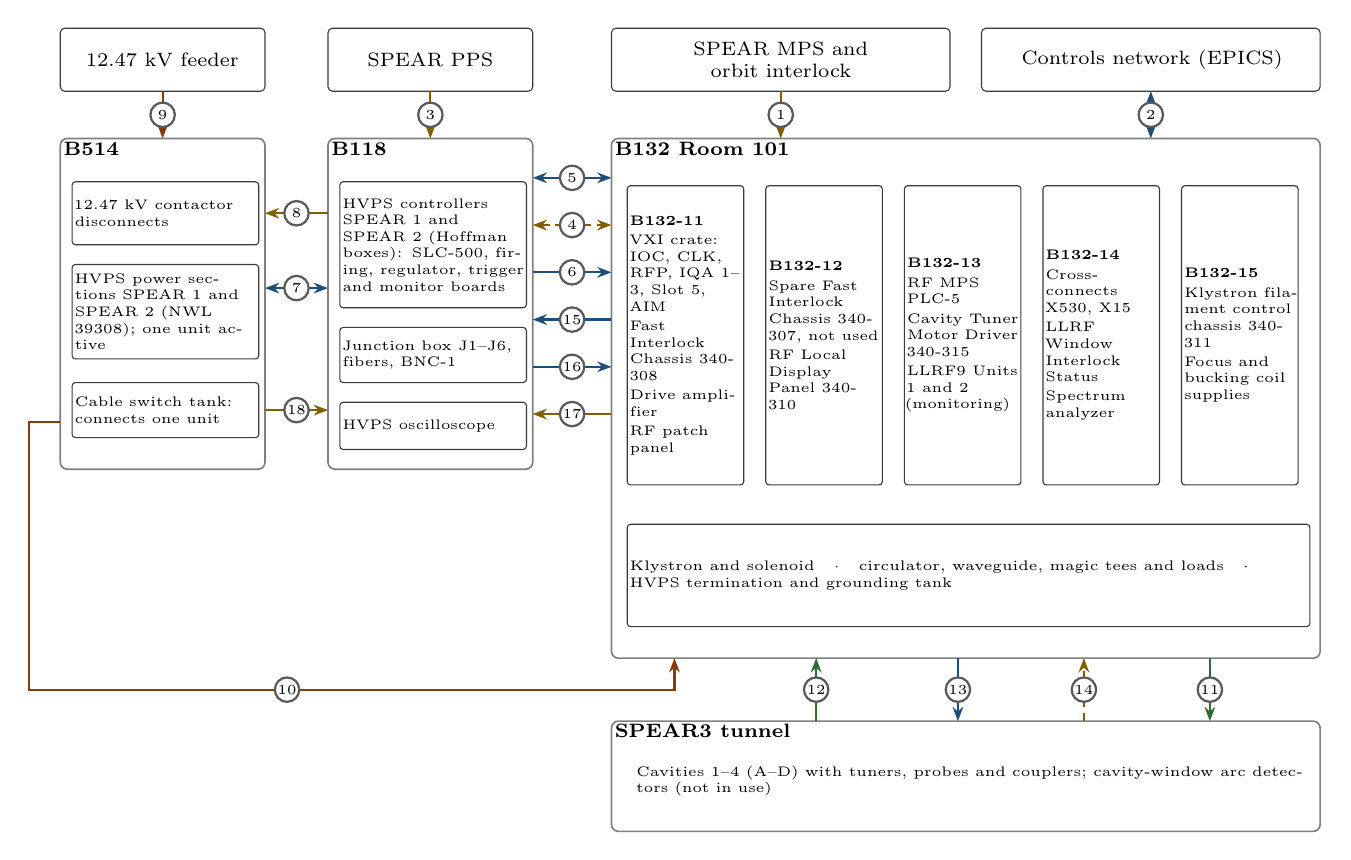
\begin{tikzpicture}[x=1mm,y=1mm,font=\scriptsize,every node/.style={outer sep=0pt},
  ext/.style={blk,anchor=north west,minimum height=8mm,inner sep=2pt},
  bldg/.style={draw=black!50,rounded corners=2.5pt,line width=0.6pt},
  ttl/.style={anchor=north west,font=\scriptsize\bfseries,inner sep=1.2pt},
  unit/.style={draw=cNeut,fill=white,rounded corners=1.2pt,anchor=north west,align=left,
               font={\tiny\uchyph=0\relax},inner sep=1pt,text width=#1},
  rack/.style={unit=14.1mm,minimum height=38mm},
  num/.style={circle,draw=black!65,fill=white,inner sep=0pt,minimum size=3.1mm,font=\tiny,solid},
  hd/.style={-{Stealth[length=1.8mm]}},
  hd2/.style={{Stealth[length=1.8mm]}-{Stealth[length=1.8mm]}},
  pw/.style={draw=cPwr,thick,hd},
  rfl/.style={draw=cRf,thick,hd},
  sg/.style={draw=cCtrl,thick,hd},
  ilk/.style={draw=cPlc,thick,hd},
  fbr/.style={draw=cPlc,thick,densely dashed},
]
% ---- outside systems ------------------------------------------------------
\node[ext,minimum width=26mm,text width=22mm] (feed) at (0,0) {12.47~kV feeder};
\node[ext,minimum width=26mm,text width=22mm] (pps)  at (34,0) {SPEAR PPS};
\node[ext,minimum width=43mm,text width=39mm] (mps)  at (70,0) {SPEAR MPS and orbit interlock};
\node[ext,minimum width=43mm,text width=39mm] (net)  at (117,0) {Controls network (EPICS)};

% ---- B514 -----------------------------------------------------------------
\draw[bldg] (0,-14) rectangle (26,-56);
\node[ttl] at (0,-14) {B514};
\node[unit=23mm,minimum height=8mm] at (1.5,-19.5) {12.47~kV contactor disconnects};
\node[unit=23mm,minimum height=12mm] at (1.5,-30) {HVPS power sections SPEAR~1 and SPEAR~2 (NWL 39308); one unit active};
\node[unit=23mm,minimum height=7mm] at (1.5,-45) {Cable switch tank: connects one unit};

% ---- B118 -----------------------------------------------------------------
\draw[bldg] (34,-14) rectangle (60,-56);
\node[ttl] at (34,-14) {B118};
\node[unit=23mm,minimum height=16mm] at (35.5,-19.5) {HVPS controllers SPEAR~1 and SPEAR~2 (Hoffman boxes): SLC-500, firing, regulator, trigger and monitor boards};
\node[unit=23mm,minimum height=7mm] at (35.5,-38) {Junction box J1--J6, fibers, BNC-1};
\node[unit=23mm,minimum height=6mm] at (35.5,-47.5) {HVPS oscilloscope};

% ---- B132 Room 101 --------------------------------------------------------
\draw[bldg] (70,-14) rectangle (160,-80);
\node[ttl] at (70,-14) {B132 Room 101};
\node[rack] at (72,-20)    {\textbf{B132-11}\\[1pt]VXI crate: IOC, CLK, RFP, IQA~1--3, Slot~5, AIM\\[1pt]Fast Interlock Chassis 340-308\\[1pt]Drive amplifier\\[1pt]RF patch panel};
\node[rack] at (89.6,-20)  {\textbf{B132-12}\\[1pt]Spare Fast Interlock Chassis 340-307, not used\\[1pt]RF Local Display Panel 340-310};
\node[rack] at (107.2,-20) {\textbf{B132-13}\\[1pt]RF MPS PLC-5\\[1pt]Cavity Tuner Motor Driver 340-315\\[1pt]LLRF9 Units 1 and~2 (monitoring)};
\node[rack] at (124.8,-20) {\textbf{B132-14}\\[1pt]Cross-connects X530, X15\\[1pt]LLRF Window Interlock Status\\[1pt]Spectrum analyzer};
\node[rack] at (142.4,-20) {\textbf{B132-15}\\[1pt]Klystron filament control chassis 340-311\\[1pt]Focus and bucking coil supplies};
\node[unit=86mm,minimum height=13mm] at (72,-63) {Klystron and solenoid\quad$\cdot$\quad circulator, waveguide, magic tees and loads\quad$\cdot$\quad HVPS termination and grounding tank};

% ---- tunnel ---------------------------------------------------------------
\draw[bldg] (70,-88) rectangle (160,-102);
\node[ttl] at (70,-88) {SPEAR3 tunnel};
\node[anchor=north west,font=\tiny,text width=86mm,align=left] at (72,-92.5)
  {Cavities 1--4 (A--D) with tuners, probes and couplers; cavity-window arc detectors (not in use)};

% ---- links (numbers as in tab:trunks) -------------------------------------
\draw[ilk] (91.5,-8) -- (91.5,-14) node[num,midway] {1};
\draw[sg,hd2] (138.5,-8) -- (138.5,-14) node[num,midway] {2};
\draw[ilk] (47,-8) -- (47,-14) node[num,midway] {3};
\draw[sg,hd2] (60,-19) -- (70,-19) node[num,midway] {5};
\draw[fbr,hd2] (60,-25) -- (70,-25) node[num,midway] {4};
\draw[sg] (60,-31) -- (70,-31) node[num,midway] {6};
\draw[sg] (70,-37) -- (60,-37) node[num,midway] {15};
\draw[sg] (60,-43) -- (70,-43) node[num,midway] {16};
\draw[ilk] (70,-49) -- (60,-49) node[num,midway] {17};
\draw[sg,hd2] (34,-33) -- (26,-33) node[num,midway] {7};
\draw[ilk] (34,-23.5) -- (26,-23.5) node[num,midway] {8};
\draw[ilk] (26,-48.5) -- (34,-48.5) node[num,midway] {18};
\draw[pw]  (13,-8) -- (13,-14) node[num,midway] {9};
\draw[pw]  (0,-50) -- (-4,-50) -- (-4,-84) -- node[num,pos=0.4] {10} (78,-84) -- (78,-80);
\draw[rfl] (146,-80) -- (146,-88) node[num,midway] {11};
\draw[rfl] (96,-88) -- (96,-80) node[num,midway] {12};
\draw[sg]  (114,-80) -- (114,-88) node[num,midway] {13};
\draw[fbr,hd] (130,-88) -- (130,-80) node[num,midway] {14};
\end{tikzpicture}

\end{fitpicture}
\caption[The legacy station by building and rack.]{The legacy station (I0) by building
and rack. Links are drawn to the building, not to the unit; the numbers refer to
\cref{tab:trunks}, which names the unit at each end. Brown: power; green: RF; blue:
control and monitor signals; olive: interlocks and permits, dashed where on fiber.
Arrows show the direction of the signals, double arrows both directions.}
\label{fig:station-overview}
\end{figure}

% generated by scripts/docw-gen.js from data/ -- do not edit
\begin{longtable}[c]{@{}F{\cw{0.52}{1.5000}}F{\cw{0.18}{1.5000}}F{\cw{0.15}{1.5000}}F{\cw{0.15}{1.5000}}@{}}
\caption{Units of the legacy station by location.}\label{tab:units-legacy}\\
\toprule
Unit & Model or drawing & Status & In service \\
\midrule
\endfirsthead
\toprule
Unit & Model or drawing & Status & In service \\
\midrule
\endhead
\bottomrule
\endlastfoot
\multicolumn{4}{@{}l}{\footnotesize\bfseries B132-11} \\
VXI crate: IOC B132-IOCRF, CLK, RFP, IQA 1–3\newline\emph{the IOC moves to new hardware at I8} & Elma 13-slot & in service & until I8 \\
Arc/Interlock Module\newline\emph{VXI slot 12} & SD-340-309-01 & in service & until I8 \\
MPS Shutoff module\newline\emph{VXI slot 5; SPEAR MPS and orbit permits in, J3 to the Fast Interlock Chassis spare-fault input} & drawing not found & in service & until I8 \\
Fast Interlock Chassis\newline\emph{below the VXI crate; kept as fallback until I8} & 340-308 & in service & until I2 \\
Drive amplifier & -- & in service & -- \\
RF patch panel & -- & in service & -- \\
\multicolumn{4}{@{}l}{\footnotesize\bfseries B132-12} \\
Fast Interlock Chassis (spare)\newline\emph{above the panel; a slightly different version, not used} & 340-307 SN04 & spare & -- \\
RF Local Display Panel\newline\emph{kept as fallback until I8} & 340-310 SN12 & in service & until I2 \\
\multicolumn{4}{@{}l}{\footnotesize\bfseries B132-13} \\
RF MPS PLC-5 (main 1771 crate and a second crate) & Allen-Bradley PLC-5 & in service & until I4 \\
Cavity Tuner Motor Driver: SLC-500 chassis with four 1746-HSTP1 modules\newline\emph{Remote I/O node 2; the motor cables move from the SS2000MD4 drivers to the Galil at I3, the chassis stays on the link and as fallback} & 340-315 SN08 & in service & until I8 \\
LLRF9 Unit 1\newline\emph{drives the station from I6} & Dimtel LLRF9 & in service (monitoring) & -- \\
LLRF9 Unit 2 & Dimtel LLRF9 & in service (monitoring) & -- \\
\multicolumn{4}{@{}l}{\footnotesize\bfseries B132-14} \\
Cross-connect X530\newline\emph{panel cable J2 on terminals 1–25 and J3 on 26–50} & -- & in service & -- \\
Cross-connect X15\newline\emph{waveguide pressure switches} & -- & in service & -- \\
LLRF Window Interlock Status chassis (2U)\newline\emph{above the spectrum analyzer; turns a legacy permit into an LLRF9 enable; replaced by the Interface Chassis at I2 (Doc C D8)} & built 2021 & in service & until I2 \\
Spectrum analyzer & -- & in service & -- \\
\multicolumn{4}{@{}l}{\footnotesize\bfseries not recorded} \\
Cross-connect X519 (PLC-5 input module) & -- & in service & -- \\
Cross-connect X522 (PLC-5 output module) & -- & in service & -- \\
Cross-connect X517 (PLC-5 analog input module 2) & -- & in service & -- \\
Cross-connect X513 (lines from the HVPS controller) & -- & in service & -- \\
24 V bus X518\newline\emph{feeds the output module and four panel spares} & -- & in service & -- \\
\multicolumn{4}{@{}l}{\footnotesize\bfseries B132-15} \\
Klystron filament control chassis & 340-311 SN14 & in service & until I5 \\
Main focus and bucking coil supplies & -- & in service & -- \\
\multicolumn{4}{@{}l}{\footnotesize\bfseries B132 Room 101} \\
Klystron and solenoid & Marconi & in service & -- \\
Circulator, waveguide, magic tees and loads & -- & in service & -- \\
HVPS termination and grounding tank\newline\emph{Ross HV grounding switch, Danfysik DC-CT (cathode current), 3.3 mΩ return shunt, Pearson CT-110} & SD-730-790-05 & in service & -- \\
\multicolumn{4}{@{}l}{\footnotesize\bfseries B118} \\
HVPS controllers SPEAR 1 and SPEAR 2 (Hoffman boxes)\newline\emph{SLC-500, Enerpro firing boards, regulator, trigger interconnect and monitor boards; one unit replaced at I7b, the other at I7c} & WD-730-790-02 & in service & until I7 \\
HVPS junction box (pluggable terminal blocks J1 to J6; fiber-optics box; BNC-1)\newline\emph{above the SPEAR 1 controller; connects the cables from B132 and B514 to the controller in service} & EI-444-636-00 & in service & -- \\
HVPS oscilloscope\newline\emph{channels: HVPS voltage, HVPS current, transformer current, SCR firing signal} & Tektronix & in service & -- \\
\multicolumn{4}{@{}l}{\footnotesize\bfseries B514} \\
HVPS power sections SPEAR 1 and SPEAR 2\newline\emph{one unit active at a time} & NWL 39308 & in service & -- \\
HVPS cable switch tank\newline\emph{connects the −90 kV output of one unit to the cable to the termination tank} & EI-444-636-00 & in service & -- \\
12.47 kV contactor disconnects & GP-439-704-02 & in service & -- \\
\multicolumn{4}{@{}l}{\footnotesize\bfseries SPEAR3 tunnel} \\
Cavities 1–4 (A–D) with tuners, probes and couplers & -- & in service & -- \\
Cavity-window arc detectors & -- & not in use & -- \\
\end{longtable}


% generated by scripts/docw-gen.js from data/ -- do not edit
\begin{longtable}[c]{@{}F{\cw{0.05}{1.6000}}F{\cw{0.23}{1.6000}}F{\cw{0.23}{1.6000}}F{\cw{0.11}{1.6000}}F{\cw{0.38}{1.6000}}@{}}
\caption{Links between buildings and to the outside (numbers as in the station overview).}\label{tab:trunks}\\
\toprule
No. & From & To & Medium & Content and drawings \\
\midrule
\endfirsthead
\toprule
No. & From & To & Medium & Content and drawings \\
\midrule
\endhead
\bottomrule
\endlastfoot
1 & SPEAR MPS and orbit interlock & VXI Slot 5 (B132-11) & wire & Two 24 V permits (J. Sebek, LLRF Interface Chassis specification); their wiring into the module is not recorded (FC2)\newline\emph{no drawing found} \\
2 & Controls network & IOC B132-IOCRF (B132-11) & Ethernet & EPICS Channel Access \\
3 & SPEAR PPS & HVPS controllers (B118) & wire & PPS 1 and PPS 2 permits\newline\emph{WD-730-790-02} \\
4 & RF Local Display Panel (B132-12) & HVPS controllers (B118) & fiber & Three fibers: SCR ENABLE, KLYSTRON CROWBAR, STATUS; through the B118 junction box to the right- and left-side interface boards of the controller in service, re-patched at a switch-over\newline\emph{WD-340-330-29; SD-730-793-07; SD-730-793-08; EI-444-636-00} \\
5 & VXI Remote I/O scanner (B132-11) & HVPS controllers (B118) & Remote I/O & SLC-500 adapter of each controller\newline\emph{WD-730-790-02} \\
6 & HVPS monitor board (B118) & RF Local Display Panel (B132-12) & wire & HVPS voltage and current monitors (TS-3 of the controller in service, cables SPR02923 and SPR02924), through J5 of the B118 junction box, X513 and X530\newline\emph{SD-730-793-12; WD-340-330-02; EI-444-636-00} \\
7 & HVPS controllers (B118) & HVPS power sections (B514) & wire & SCR firing, 12 pairs to the phase-tank thyristor stacks; crowbar and voltage-divider cables\newline\emph{WD-730-790-01; WD-730-794-04} \\
8 & HVPS controllers (B118) & Contactor disconnects (B514) & wire & TS-5, 15 terminals (Belden 83715): contactor on/off (MX coil), K-4 PPS control relay, RR remote reset relay\newline\emph{WD-730-790-01; WD-730-794-02} \\
9 & 12.47 kV feeder & Contactor disconnects (B514) & power & 12.47 kV AC to the power sections\newline\emph{GP-439-704-02; ID-308-801-06} \\
10 & HVPS power sections (B514) & Termination tank and klystron (B132) & HV cable & −90 kV DC: each unit's output to the cable switch tank in B514, which connects one unit; from it SPR02925 (−90 kV) and SPR02926 (ground) to the termination tank\newline\emph{EI-444-636-00; WD-730-790-01; SD-730-790-05} \\
11 & Circulator and waveguide (B132) & Cavities (tunnel) & waveguide & RF power \\
12 & Cavity probes and couplers (tunnel) & RF patch panel (B132-11) & coax & RF monitor signals\newline\emph{SD-340-330-01} \\
13 & SS2000MD4 tuner motor drivers (B132) & Tuner motors (tunnel) & wire & Stepper motor cables \\
14 & Arc detectors (tunnel) & Fast Interlock Chassis (B132-11) & fiber & Arc-detector fibers (cavity-window detectors not in use)\newline\emph{SD-340-308-02} \\
15 & Termination tank (B132 Room 101) & HVPS controllers (B118) & wire and coax & Through the B118 junction box to the controller in service: SPR02944 and SPR02945 to TS-6 (terminals 9 to 14 and 1 to 6); SPR02946 for the oil-level switch LEV-3; SPR02947 coax from BNC-1 (klystron arc) to the left-side interface board. On TS-6: return-cable shunt on 20 and 21 to BNC-12, grounding-switch auxiliary contact on 11 and 12 (PPS chain 2 readback); Pearson CT-110 to J1 of SD-730-793-08. DC-CT output route not recorded\newline\emph{EI-444-636-00; WD-730-790-01; SD-730-790-05} \\
16 & HVPS monitor boards (B118) & AIM (VXI slot 12; B132-11) & wire & 9-conductor cable from the DB9 of the monitor board SD-730-793-12 of the controller in service, through J3 of the B118 junction box, to the AIM's DB9\newline\emph{EI-444-636-00} \\
17 & Pressure switch and PLC-5 (B132) & HVPS controllers (B118) & wire & Through J4 of the B118 junction box to TS-1 of the touch panel of the controller in service: a pressure switch labeled W6 PRESS, a flashing light, and PLC DC common from the PLC-5 DCM module\newline\emph{EI-444-636-00} \\
18 & Flow switch beside the cable switch tank (B514) & HVPS controllers (B118) & wire & Two wires through J6 of the B118 junction box to TS-4 terminals 13 and 14 of the controller in service\newline\emph{EI-444-636-00} \\
\end{longtable}


% ===========================================================================
\section{Drawing Register}\label{sec:register}

The register lists every drawing file in the drawing folders of the repository:
\fpath{hvps/documentation/} (schematics, stack assemblies, switchgear and wiring
diagrams), \fpath{llrf/documentation/} (coaxial cables, filament heater, the PEP-II
block diagrams and system descriptions, the legacy interface modules, the RF Local
Display Panel and the RF MPS wiring diagrams) and \fpath{pps/}, and the HVPS technical
specification in \fpath{hvps/architecture/originalDocuments/}. It holds \WDrawings{}
drawings (\cref{tab:drawing-summary}): \WStatusList. A drawing is verified against
another drawing, the PLC program, the EPICS database, a photograph or measurement of
the hardware, or an account of the installed system by the RF group (F.~Wang's
confirmation or J.~Sebek's notes); the notes say which. Where the
repository holds more than one copy of a drawing, all are listed. The last column of
\cref{tab:drawings} gives the documents that cite the drawing, by number or by file
name.

% generated by scripts/docw-gen.js from data/ -- do not edit
\begin{longtable}[c]{@{}F{\cw{0.24}{1.7143}}F{\cw{0.12}{1.7143}}F{\cw{0.128}{1.7143}}F{\cw{0.128}{1.7143}}F{\cw{0.128}{1.7143}}F{\cw{0.128}{1.7143}}F{\cw{0.128}{1.7143}}@{}}
\caption{Drawing status by area.}\label{tab:drawing-summary}\\
\toprule
Area & Drawings & verified & errata & disputed & reference & PEP-II \\
\midrule
\endfirsthead
\toprule
Area & Drawings & verified & errata & disputed & reference & PEP-II \\
\midrule
\endhead
\bottomrule
\endlastfoot
HVPS & 30 & 15 & 5 & -- & 10 & -- \\
Switchgear & 5 & 4 & -- & -- & 1 & -- \\
LLRF & 1 & -- & -- & -- & -- & 1 \\
Heater & 1 & 1 & -- & -- & -- & -- \\
Architecture & 14 & -- & -- & -- & -- & 14 \\
Interface modules & 3 & 3 & -- & -- & -- & -- \\
Local panel & 13 & 7 & -- & 1 & 5 & -- \\
RF MPS & 33 & 15 & 15 & -- & -- & 3 \\
PPS & 3 & -- & -- & -- & 3 & -- \\
\midrule
Total & 103 & 45 & 20 & 1 & 19 & 18 \\
\end{longtable}


% generated by scripts/docw-gen.js from data/ -- do not edit
\begin{longtable}[c]{@{}F{\cw{0.17}{1.6000}}F{\cw{0.51}{1.6000}}F{\cw{0.11}{1.6000}}F{\cw{0.09}{1.6000}}F{\cw{0.12}{1.6000}}@{}}
\caption{Drawing register.}\label{tab:drawings}\\
\toprule
Drawing & Title, notes and file & Status & Errata & Cited in \\
\midrule
\endfirsthead
\toprule
Drawing & Title, notes and file & Status & Errata & Cited in \\
\midrule
\endhead
\bottomrule
\endlastfoot
\multicolumn{5}{@{}l}{\footnotesize\bfseries HVPS} \\
PS-341-360-01 rev~02 & PEP-II RF system: 2.5 MW klystron power supply, technical specification\newline\emph{R. Cassel, Power Conversion Department, January 2004 (title page R2). A specification, not a drawing; no wiring. Doc 0 replaces its §1.5 phase-shifting transformer rating, 350 kVA, with the 2750 kVA nameplate of EI-730-790-00}\newline \dpath{hvps/architecture/originalDocuments/ps3413600102.pdf} & reference &  & 0, L, P \\
SD-237-230-12 rev~00 & Enerpro general-purpose three-phase firing circuit, PCB FCOG6100 (Enerpro E128)\newline\emph{PP1 jumper block: phase reference (1–6) and gate-pulse profile (7–8). Agrees with J. Sebek's note on the installed board (R37 to R39 200 kΩ)}\newline \dpath{hvps/documentation/schematics/sd2372301200.pdf} & verified &  & L \\
SD-237-230-14 rev~01 & Analog regulator card\newline\emph{Compared with J. Sebek's regulator-board notes and the HVPS ladder program (N7:10 to output 0 of the NIO4V in slot 8)}\newline \dpath{hvps/documentation/schematics/sd2372301401.pdf} & errata & E19 & 0, L \\
SD-730-790-01 rev~01 & HVPS system schematic (top level)\newline\emph{Agrees with NWL's schematic EI-730-790-00, except that its input label rounds the 2750 kVA nameplate to 3000 kVA}\newline \dpath{hvps/documentation/schematics/sd7307900101.pdf} & verified &  & 0, L \\
SD-730-790-05 rev~01 & Grounding tank schematic\newline\emph{Termination inductors 350 µH as built. J1 (MS3102R18-1P) agrees with WD-730-794-06}\newline \dpath{hvps/documentation/schematics/sd7307900501.pdf}\newline copy: \dpath{pps/sd7307900501.pdf} & verified &  & L \\
SD-730-791-03 rev~00 & High-voltage SCR gate trigger board\newline\emph{Board circuit of the stack-mounted gate trigger board (1996); no inter-unit wiring}\newline \dpath{hvps/documentation/stackAssemblies/StackDriver1sd73079103.pdf} & reference &  & -- \\
SD-730-793-03 rev~04 & 2 MW klystron PS 12 kV SCR driver board\newline\emph{Its 16 µs gate pulses and P1 rails (240 V, 120 V) agree with J. Sebek's HVPS hazards note}\newline \dpath{hvps/documentation/schematics/sd7307930304.pdf} & verified &  & L \\
SD-730-793-04 rev~02 & SCR crowbar trigger board (2002 version)\newline\emph{Supersedes SD-730-794-04. P1 as on SD-730-793-03 and -13}\newline \dpath{hvps/documentation/schematics/sd7307930402.pdf} & verified &  & L \\
SD-730-793-07 rev~02 & Right-side trigger interconnect board\newline\emph{SCR ENABLE fiber on J2, as on WD-340-330-29 and EI-444-636-00}\newline \dpath{hvps/documentation/schematics/sd7307930702.pdf} & verified &  & L, M \\
SD-730-793-08 rev~01 & Left-side trigger interconnect board\newline\emph{KLYSTRON CROWBAR and STATUS fibers on J2 and J3 and the klystron-arc BNC J1, as on WD-340-330-29 and EI-444-636-00}\newline \dpath{hvps/documentation/schematics/sd7307930801.pdf} & verified &  & L, M \\
SD-730-793-12 rev~03 & HVPS monitor board\newline\emph{Buffers the HVPS voltage and current sent to B132. Its DB9 agrees with EI-444-636-00, and its 10 kV/V scale with the divider WD-730-794-04 and the June 2020 readback}\newline \dpath{hvps/documentation/schematics/sd7307931203.pdf} & verified &  & 0, C, L \\
SD-730-793-13 rev~01 & 2 MW klystron PS optical SCR trigger board\newline\emph{Its 16 µs gate pulses agree with J. Sebek's HVPS hazards note; P1 as on SD-730-793-03}\newline \dpath{hvps/documentation/schematics/sd7307931301.pdf} & verified &  & L \\
SD-730-794-04 rev~00 & SCR crowbar trigger board (1999 version)\newline\emph{Superseded by SD-730-793-04: the same function and P1 connector}\newline \dpath{hvps/documentation/schematics/sd7307940400.pdf} & verified &  & L \\
AD-730-792-01 rev~00 & 15 kV SCR assembly\newline\emph{Mechanical; no wiring; parts include PF-730-792-13 and -17}\newline \dpath{hvps/documentation/stackAssemblies/ad7307920100.pdf} & reference &  & -- \\
AD-730-792-08 rev~00 & Crowbar tank: light crowbar assembly\newline\emph{Mechanical; no wiring}\newline \dpath{hvps/documentation/stackAssemblies/ad7307920800.pdf} & reference &  & -- \\
AD-730-794-16 rev~00 & Klystron diode assembly, 50 kV\newline\emph{Mechanical; no wiring}\newline \dpath{hvps/documentation/stackAssemblies/ad7307941600.pdf} & reference &  & -- \\
PF-730-792-13 rev~00 & 15 kV AC SCR: cast SCR support\newline\emph{Mechanical; no wiring; part of AD-730-792-01}\newline \dpath{hvps/documentation/stackAssemblies/pf7307921300.pdf} & reference &  & -- \\
PF-730-792-17 rev~02 & 15 kV SCR: SCR end part\newline\emph{Mechanical; no wiring; part of AD-730-792-01 and -08 and AD-730-794-15 and -16}\newline \dpath{hvps/documentation/stackAssemblies/pf7307921702.pdf} & reference &  & -- \\
PF-730-792-22 rev~00 & 15 kV AC SCR crowbar: tension rod, 25 in\newline\emph{Mechanical; no wiring; part of AD-730-792-02}\newline \dpath{hvps/documentation/stackAssemblies/pf7307922200.pdf} & reference &  & -- \\
PF-730-792-29 rev~00 & Crowbar tank: tension rod, 20.75 in\newline\emph{Mechanical; no wiring; part of AD-730-792-01 and AD-730-794-16}\newline \dpath{hvps/documentation/stackAssemblies/pf7307922900.pdf} & reference &  & -- \\
PF-730-793-22 rev~01 & 15 kV AC light SCR: tension rod, 11.5 in\newline\emph{Mechanical; no wiring; part of AD-730-792-08}\newline \dpath{hvps/documentation/stackAssemblies/pf7307932201.pdf} & reference &  & -- \\
EI-444-636-00 rev~01 & SPEAR3 2.5 MW klystron power supply system: electrical interconnect (3 sheets)\newline\emph{Matches the installed system (F. Wang, 11 November 2026). The source of links 4, 6, 10 and 15 to 18}\newline \dpath{hvps/documentation/wiringDiagrams/ei4446360001.pdf} & errata & E16 E17 E18 & -- \\
EI-730-790-00 rev~00 & Klystron power supply electrical schematic (NWL 39308)\newline\emph{The transformer manufacturer's schematic. Its switches agree with WD-730-794-05}\newline \dpath{hvps/documentation/wiringDiagrams/ei7307900000.pdf} & verified &  & 0, L \\
WD-730-790-01 rev~03 & Interconnection wiring: B118 controller, contactor disconnect, termination tank\newline \dpath{hvps/documentation/wiringDiagrams/wd7307900103.pdf}\newline copy: \dpath{pps/wd7307900103.pdf} & errata & E2 & L \\
WD-730-790-02 rev~06 & Trigger enclosure wiring (B118 HVPS controller)\newline\emph{Master wiring diagram of the controller. Its I/O labels agree with the HVPS ladder program, and its SLC 5/03 processor in slot 0 is the one installed (F. Wang, 11 November 2026)}\newline \dpath{hvps/documentation/wiringDiagrams/wd7307900206.pdf}\newline copy: \dpath{pps/wd7307900206.pdf} & verified &  & 0, L \\
WD-730-794-02 rev~00 & SCR control driver, contactor interconnecting cables\newline\emph{TS-5 conductor list}\newline \dpath{hvps/documentation/wiringDiagrams/wd7307940200.pdf} & errata & E3 & L \\
WD-730-794-03 rev~00 & SCR control driver: SCR interconnecting cables\newline\emph{Twelve SCR gate cables from the transformer tank (WD-730-792-01) to trigger boards H1 and H2, through P1 and P2 on 30 ft cables; thermocouples TC-1, TC-2 and oil level LEV1 to TS-6. Belden 88761 pairs as on WD-730-790-01}\newline \dpath{hvps/documentation/wiringDiagrams/wd7307940300.pdf} & verified &  & -- \\
WD-730-794-04 rev~00 & SCR control driver, crowbar interconnecting cables\newline\emph{Includes the transformer tank (WD-730-792-01) and the output voltage dividers, whose ratio agrees with the monitor board SD-730-793-12 (10 kV/V) and the June 2020 readback}\newline \dpath{hvps/documentation/wiringDiagrams/wd7307940400.pdf} & verified &  & 0, L \\
WD-730-794-05 rev~03 & SCR control driver: transformer cables\newline\emph{NWL termination box (pressure and vacuum, oil over-temperature, oil level, pressure relief, oil flow; CTs) to the Hoffman box; the same switches as EI-730-790-00}\newline \dpath{hvps/documentation/wiringDiagrams/wd7307940503.pdf} & verified &  & -- \\
WD-730-794-06 rev~00 & Grounding tank wiring (test-stand configuration)\newline\emph{No revisions recorded}\newline \dpath{hvps/documentation/wiringDiagrams/wd7307940600.pdf}\newline copy: \dpath{pps/wd7307940600.pdf} & errata & E9 & L \\
\multicolumn{5}{@{}l}{\footnotesize\bfseries Switchgear} \\
GP-308-500-01 rev~03 & 12.47 kV vacuum contactor controller, schematic and general arrangement (LBL, 1977)\newline\emph{Authoritative relay legend; it names the relays of the as-built schematic GP-439-704-02 (MX, RR, TX)}\newline \dpath{hvps/documentation/switchgear/gp3085000103.pdf} & verified &  & 0, I, L \\
GP-439-704-02 rev~01 & Vacuum contactor controller electrical schematic (as built, 2006)\newline\emph{Agrees with ID-308-801-06 and Ross 713203 on the PPS readback path (TB3-22 to 24)}\newline \dpath{hvps/documentation/switchgear/gp4397040201.pdf}\newline copy: \dpath{pps/gp4397040201.pdf} & verified &  & 0, I, L \\
ID-308-801-06 rev~01 & 12.47 kV vacuum contactor controller, connection wiring (as built, 2006)\newline\emph{Agrees with GP-439-704-02 and Ross 713203 on the PPS readback path}\newline \dpath{hvps/documentation/switchgear/id3088010601.pdf} & verified &  & 0, I, L \\
Ross 713203 rev~E & Vacuum contactor energy-storage closing and holding system (HCA-1-A driver, HQ3 contactor)\newline\emph{Vendor drawing. Agrees with ID-308-801-06 and GP-439-704-02 on the PPS readback path (auxiliary contact S5 on TB2-18 to 20)}\newline \dpath{hvps/documentation/switchgear/rossEngr713203.pdf}\newline copy: \dpath{pps/rossEngr713203.pdf} & verified &  & 0, L \\
ABB DB 41-122M & ABB descriptive bulletin: Type MCO microprocessor time-overcurrent relay (devices 50/51), August 1996\newline\emph{Vendor data, not a drawing; MCO relays are named on GP-439-704-02}\newline \texttt{\scriptsize hvps/documentation/switchgear/DB41-122m\ \ \ \ MCO.pdf} & reference &  & -- \\
\multicolumn{5}{@{}l}{\footnotesize\bfseries LLRF} \\
SD-340-330-01 rev~00 & Coax cable plant\newline\emph{PEP-II four-cavity coax cable plant (forward, reflected and probe of cavities A to D, klystron, circulator and loads); the SPEAR3 jacks are field check FC8}\newline \dpath{llrf/documentation/coaxCables/sd3403300100.pdf} & PEP-II &  & L \\
\multicolumn{5}{@{}l}{\footnotesize\bfseries Heater} \\
SD-340-311-00 rev~02 & Klystron filament control chassis (340-311)\newline\emph{J1 agrees with WD-340-330-28 (filament on, motor up) and WD-340-330-21 (voltage and current monitors on terminals 11 and 12, channels 9 and 10)}\newline \dpath{llrf/documentation/filamentHeater/sd3403110002.pdf} & verified &  & 0, L, M \\
\multicolumn{5}{@{}l}{\footnotesize\bfseries Architecture} \\
BD-340-330-00 rev~00 & PEP-II LER RF station block diagram\newline\emph{PEP-II LER station LR44 with two cavities (P. Corredoura, January 1999); cited for the panel's beam-abort output}\newline \dpath{llrf/documentation/legacyArchitecture/bd3403300000.pdf} & PEP-II &  & C, I, L, M \\
BD-340-330-01 rev~00 & LLRF block diagram (alternative view)\newline\emph{PEP-II LER LLRF configuration (two cavities)}\newline \dpath{llrf/documentation/legacyArchitecture/bd3403300100.pdf} & PEP-II &  & L \\
BD-340-329-01 rev~00 & PEP-II HER LLRF configuration, block diagram\newline\emph{PEP-II HER LLRF configuration (four cavities), February 1999; includes loops not installed at SPEAR3}\newline \dpath{llrf/documentation/legacyArchitecture/blockDiagrambd3403290100-1.pdf} & PEP-II &  & -- \\
PS-340-330-51 rev~00 & PEP-II RF system description (Schwarz)\newline\emph{PEP-II system description; background in Docs L and P}\newline \dpath{llrf/documentation/legacyArchitecture/ps3403305100.pdf} & PEP-II &  & L, P \\
PS-340-330-52 rev~00 & LLRF feedback loop description (Schwarz)\newline\emph{PEP-II feedback loops; background in Docs L and P}\newline \dpath{llrf/documentation/legacyArchitecture/feedbackLoopDescriptionps3403305200.pdf} & PEP-II &  & L, P \\
PS-340-330-53 rev~00 & RF cavity low-power calibration procedure\newline\emph{PEP-II procedure (H. Schwarz), July 1999}\newline \dpath{llrf/documentation/legacyArchitecture/ps3403305300.pdf} & PEP-II &  & -- \\
PS-340-330-54 rev~00 & RF station safety certification check-off list\newline\emph{PEP-II procedure, July 1999}\newline \dpath{llrf/documentation/legacyArchitecture/ps3403305400.pdf} & PEP-II &  & -- \\
PS-340-330-55 rev~03 & RF station safety survey\newline\emph{PEP-II, revised December 2005}\newline \dpath{llrf/documentation/legacyArchitecture/ps3403305503.pdf} & PEP-II &  & -- \\
PS-340-330-56 rev~00 & RF station coupling and cable calibration procedure\newline\emph{PEP-II procedure, July 1999}\newline \dpath{llrf/documentation/legacyArchitecture/ps3403305600.pdf} & PEP-II &  & -- \\
PS-340-330-57 rev~00 & RF station full-power test and survey\newline\emph{PEP-II procedure, July 1999}\newline \dpath{llrf/documentation/legacyArchitecture/ps3403305700.pdf} & PEP-II &  & -- \\
PS-340-330-58 rev~00 & RF station cavity phasing procedure\newline\emph{PEP-II procedure, July 1999}\newline \dpath{llrf/documentation/legacyArchitecture/ps3403305800.pdf} & PEP-II &  & -- \\
PS-340-330-59 rev~00 & RF station turn-on procedure\newline\emph{PEP-II procedure, July 1999}\newline \dpath{llrf/documentation/legacyArchitecture/ps3403305900.pdf} & PEP-II &  & -- \\
PS-340-330-60 rev~01 & Bellow cavity phasing procedure\newline\emph{PEP-II procedure, September 1999}\newline \dpath{llrf/documentation/legacyArchitecture/ps3403306001.pdf} & PEP-II &  & -- \\
PS-340-330-61 rev~02 & RF non-ionizing radiation safety procedure\newline\emph{PEP-II procedure, January 2000}\newline \dpath{llrf/documentation/legacyArchitecture/ps3403306102.pdf} & PEP-II &  & -- \\
\multicolumn{5}{@{}l}{\footnotesize\bfseries Interface modules} \\
SD-340-308-01 rev~R1 & Fast Interlock Chassis, transmitter board (command fibers)\newline\emph{Chassis 340-308 in service; its fiber jacks J45 to J50 agree with the rear photograph. The scan cuts off the number field: number and revision are from the file name}\newline \dpath{llrf/documentation/legacyInterfaceModules/SD-340-308-01-R1-1of1.pdf} & verified &  & C, I, L, M \\
SD-340-308-02 rev~R1 & Fast Interlock Chassis, receiver board (J15, J2, detector)\newline\emph{J15 and J2 agree pin for pin with the AIM schematic SD-340-309-01}\newline \dpath{llrf/documentation/legacyInterfaceModules/SD-340-308-02-R1.pdf} & verified &  & C, I, L, M \\
SD-340-309-01 rev~02 & Arc/Interlock Module (AIM)\newline\emph{2018 redraw. J3 and J4 agree pin for pin with SD-340-308-02; the enable word read in EPICS (0x71FB, 11 November 2026) fits its jumper logic on sheet 14}\newline \dpath{llrf/documentation/legacyInterfaceModules/sd3403090102.pdf} & verified &  & 0, C, I, L, M \\
\multicolumn{5}{@{}l}{\footnotesize\bfseries Local panel} \\
AD-340-310-00 rev~00 & RF Local Display Panel assembly, with the front-panel lamp layout\newline\emph{Lamp layout agrees with the legend SI-340-310-05 and the panel in service (340-310 SN12, photograph)}\newline \dpath{llrf/documentation/localPanel/ad3403100000.pdf} & verified &  & -- \\
AD-340-310-05 rev~00 & RF Local Display Panel assembly, -05 version\newline\emph{Lamp layout agrees with the legend SI-340-310-05 and the panel in service (photograph)}\newline \dpath{llrf/documentation/localPanel/ad3403100500.pdf} & verified &  & -- \\
DL-340-310-00 rev~00 & RF Local Display Panel drawing list\newline\emph{Lists twelve drawings of the panel set; all twelve are in the repository}\newline \dpath{llrf/documentation/localPanel/dl3403100000.pdf} & verified &  & I, L, M \\
GP-340-310-01 rev~00 & RF Local Display Panel PC card layout\newline\emph{PC card layout (lamp positions D2 to D44); no inter-unit wiring}\newline \dpath{llrf/documentation/localPanel/gp3403100100.pdf} & reference &  & -- \\
ML-340-310-00 rev~00 & RF Local Display Panel material list\newline\emph{J2 female and J3 male (page 2), as on SD-340-311-01}\newline \dpath{llrf/documentation/localPanel/ml3403100000.pdf} & verified &  & -- \\
PC-340-310-01 rev~00 & RF Local Display Panel PC card dimensions\newline\emph{PC card dimensions; no wiring}\newline \dpath{llrf/documentation/localPanel/pc3403100100.pdf} & reference &  & -- \\
PF-340-310-01 rev~00 & RF Local Display Panel front panel, 15 3/4 in (fabrication)\newline\emph{Fabrication; no wiring}\newline \dpath{llrf/documentation/localPanel/pf3403100100.pdf} & reference &  & -- \\
PF-340-310-02 rev~00 & RF Local Display Panel rear panel (fabrication)\newline\emph{Fabrication; connector cut-outs per SC-125-050-21}\newline \dpath{llrf/documentation/localPanel/pf3403100200.pdf} & reference &  & -- \\
PF-340-310-05 rev~02 & RF Local Display Panel front panel (fabrication), revised\newline\emph{Fabrication; revisions added a hole and a dimension}\newline \dpath{llrf/documentation/localPanel/pf3403100502.pdf} & reference &  & -- \\
SD-340-311-01 rev~00 & RF Local Display Panel schematic (PEP-II RF System Local Panel)\newline\emph{J2 AMP 745078-3 (female); J3 AMP 745078-1 (male)}\newline \dpath{llrf/documentation/localPanel/sd3403110100.pdf} & disputed & E4 & C, I, L, M \\
SI-340-310-01 rev~00 & RF Local Display Panel front-panel legend\newline\emph{Legend agrees with SI-340-310-05 and the panel in service (photograph)}\newline \dpath{llrf/documentation/localPanel/si3403100100.pdf} & verified &  & -- \\
SI-340-310-02 rev~00 & RF Local Display Panel rear panel\newline\emph{Matches the rear photograph}\newline \dpath{llrf/documentation/localPanel/si3403100200.pdf} & verified &  & I, L, M \\
SI-340-310-05 rev~01 & RF Local Display Panel front panel\newline\emph{Legend agrees label for label with the panel in service (340-310 SN12, photograph)}\newline \dpath{llrf/documentation/localPanel/si3403100501.pdf} & verified &  & I, L, M \\
\multicolumn{5}{@{}l}{\footnotesize\bfseries RF MPS} \\
WD-340-330-02 rev~00 & Wiring to the RF Local Display Panel (cross-connect X530)\newline \dpath{llrf/documentation/mpsWiringDiagrams/wd3403300200.pdf} & errata & E4 E5 E7 & C, I, L, M \\
WD-340-330-03 rev~00 & Cavity junction boxes A to D: tuner limit switches, flow switches, position pots, IR detectors, tuner motor phases\newline\emph{J. Sebek's LLRF notes ask for its A-B module labels to be corrected}\newline \dpath{llrf/documentation/mpsWiringDiagrams/wd3403300300.pdf} & errata & E10 & -- \\
WD-340-330-04 rev~00 & Cavity vacuum: gauge controllers and ion-pump supplies of cavities A to D\newline\emph{Inputs agree with the PLC-5 program (I:032/1, /4, /11, /14 and I:033/1, /4, /11, /14)}\newline \dpath{llrf/documentation/mpsWiringDiagrams/wd3403300400.pdf} & verified &  & -- \\
WD-340-330-05 rev~00 & Waveguide air (NIRP) interlock\newline\emph{Does not match SPEAR3 (J. Sebek)}\newline \dpath{llrf/documentation/mpsWiringDiagrams/wd3403300500.pdf} & PEP-II &  & -- \\
WD-340-330-06 rev~01 & Waveguide air (NIRP) interlock\newline\emph{Does not match SPEAR3 (J. Sebek)}\newline \dpath{llrf/documentation/mpsWiringDiagrams/wd3403300601.pdf} & PEP-II &  & -- \\
WD-340-330-07 rev~00 & PLC-5 thermocouple module 1 (1771-IXE): klystron collector, body, water and window air\newline\emph{Channel names agree with the legacy EPICS database (rf\_\allowbreak{}temp\_\allowbreak{}All and rf\_\allowbreak{}temp\_\allowbreak{}4CV substitutions), DCM table 2 words 4 to 11}\newline \dpath{llrf/documentation/mpsWiringDiagrams/wd3403300700.pdf} & verified &  & -- \\
WD-340-330-08 rev~00 & Thermocouple module 2: return water of the waveguide loads and the circulator\newline\emph{Other channels agree with EPICS: crate power supply, ambient air, RF (drive) amplifier, circulator and three load HCW returns}\newline \dpath{llrf/documentation/mpsWiringDiagrams/wd3403300800.pdf} & errata & E14 & -- \\
WD-340-330-09 rev~00 & Thermocouple module 3: cavity A body 1 to 8\newline\emph{Channel names agree with the legacy EPICS database (rf\_\allowbreak{}temp\_\allowbreak{}All and rf\_\allowbreak{}temp\_\allowbreak{}4CV substitutions)}\newline \dpath{llrf/documentation/mpsWiringDiagrams/wd3403300900.pdf} & verified &  & -- \\
WD-340-330-10 rev~00 & Thermocouple module 4: cavity A body 9 to 14 and tuners\newline\emph{Channel names agree with the legacy EPICS database (rf\_\allowbreak{}temp\_\allowbreak{}All and rf\_\allowbreak{}temp\_\allowbreak{}4CV substitutions)}\newline \dpath{llrf/documentation/mpsWiringDiagrams/wd3403301000.pdf} & verified &  & -- \\
WD-340-330-11 rev~00 & Thermocouple module 5: cavity A HOM loads, water, tuner bellows and spare\newline\emph{Channel names agree with the legacy EPICS database (rf\_\allowbreak{}temp\_\allowbreak{}All and rf\_\allowbreak{}temp\_\allowbreak{}4CV substitutions), except channel 8 (E15)}\newline \dpath{llrf/documentation/mpsWiringDiagrams/wd3403301100.pdf} & errata & E15 & -- \\
WD-340-330-12 rev~00 & Thermocouple module 6: cavity B body 1 to 8\newline\emph{Channel names agree with the legacy EPICS database (rf\_\allowbreak{}temp\_\allowbreak{}All and rf\_\allowbreak{}temp\_\allowbreak{}4CV substitutions)}\newline \dpath{llrf/documentation/mpsWiringDiagrams/wd3403301200.pdf} & verified &  & -- \\
WD-340-330-13 rev~00 & Thermocouple module 7: cavity B body 9 to 14 and tuners\newline\emph{Channel names agree with the legacy EPICS database (rf\_\allowbreak{}temp\_\allowbreak{}All and rf\_\allowbreak{}temp\_\allowbreak{}4CV substitutions)}\newline \dpath{llrf/documentation/mpsWiringDiagrams/wd3403301300.pdf} & verified &  & -- \\
WD-340-330-14 rev~00 & Thermocouple module 8: cavity B HOM loads, tuner bellows and spare\newline\emph{Channel names agree with the legacy EPICS database (rf\_\allowbreak{}temp\_\allowbreak{}All and rf\_\allowbreak{}temp\_\allowbreak{}4CV substitutions), except channel 8 (E15)}\newline \dpath{llrf/documentation/mpsWiringDiagrams/wd3403301400.pdf} & errata & E15 & -- \\
WD-340-330-15 rev~00 & Thermocouple module 9: cavity C body 1 to 8\newline\emph{Channel names agree with the legacy EPICS database (rf\_\allowbreak{}temp\_\allowbreak{}All and rf\_\allowbreak{}temp\_\allowbreak{}4CV substitutions)}\newline \dpath{llrf/documentation/mpsWiringDiagrams/wd3403301500.pdf} & verified &  & -- \\
WD-340-330-16 rev~00 & Thermocouple module 10: cavity C body 9 to 14 and tuner\newline\emph{Channel names agree with the legacy EPICS database (rf\_\allowbreak{}temp\_\allowbreak{}All and rf\_\allowbreak{}temp\_\allowbreak{}4CV substitutions)}\newline \dpath{llrf/documentation/mpsWiringDiagrams/wd3403301600.pdf} & verified &  & -- \\
WD-340-330-17 rev~00 & Thermocouple module 11: cavity C HOM loads, water, tuner bellows and spare\newline\emph{Channel names agree with the legacy EPICS database (rf\_\allowbreak{}temp\_\allowbreak{}All and rf\_\allowbreak{}temp\_\allowbreak{}4CV substitutions), except channel 8 (E15); the module is labeled MODULE 11 (E20)}\newline \dpath{llrf/documentation/mpsWiringDiagrams/wd3403301700.pdf} & errata & E15 E20 & -- \\
WD-340-330-18 rev~00 & Thermocouple module 12: cavity D body 1 to 8\newline\emph{Channel names agree with the legacy EPICS database (rf\_\allowbreak{}temp\_\allowbreak{}All and rf\_\allowbreak{}temp\_\allowbreak{}4CV substitutions)}\newline \dpath{llrf/documentation/mpsWiringDiagrams/wd3403301800.pdf} & verified &  & -- \\
WD-340-330-19 rev~00 & Thermocouple module 13: cavity D body 9 to 14 and tuner\newline\emph{Channel names agree with the legacy EPICS database (rf\_\allowbreak{}temp\_\allowbreak{}All and rf\_\allowbreak{}temp\_\allowbreak{}4CV substitutions); the module is labeled MODULE 25 (E20)}\newline \dpath{llrf/documentation/mpsWiringDiagrams/wd3403301900.pdf} & errata & E20 & -- \\
WD-340-330-20 rev~00 & Thermocouple module 14: cavity D HOM loads, tuner bellows and spare\newline\emph{Channel names agree with the legacy EPICS database (rf\_\allowbreak{}temp\_\allowbreak{}All and rf\_\allowbreak{}temp\_\allowbreak{}4CV substitutions), except channel 8 (E15)}\newline \dpath{llrf/documentation/mpsWiringDiagrams/wd3403302000.pdf} & errata & E15 & -- \\
WD-340-330-21 rev~00 & PLC-5 analog input module 1\newline\emph{Filament voltage and current on terminals 11 and 12 (channels 9 and 10), as on the filament chassis SD-340-311-00 and WD-340-330-28; terminals 13, 14 and 16 agree with WD-340-330-32; the channel order agrees with the EPICS database}\newline \dpath{llrf/documentation/mpsWiringDiagrams/wd3403302100.pdf} & verified &  & C, M \\
WD-340-330-22 rev~00 & PLC-5 analog input module 2\newline\emph{The channel order agrees with the EPICS database; RF power level on terminal 12 (channel 10)}\newline \dpath{llrf/documentation/mpsWiringDiagrams/wd3403302200.pdf} & errata & E6 & C, M \\
WD-340-330-23 rev~00 & PLC-5 digital input module 1 (1771-IBN, rack X4 module 9)\newline \dpath{llrf/documentation/mpsWiringDiagrams/wd3403302300.pdf} & errata & E6 E7 E21 E22 & C, I, M \\
WD-340-330-24 rev~00 & PLC-5 digital input module 2 (2 sheets): cavity vacuum and flow interlocks\newline\emph{Cavity flow, vacuum and ion-pump current inputs (through X520) agree with the program (I:032/0, /1, /4, /10, /11, /14 and I:033/0, /1, /4, /10, /11, /14) and with WD-340-330-03 and -04}\newline \dpath{llrf/documentation/mpsWiringDiagrams/wd3403302400.pdf} & verified &  & -- \\
WD-340-330-25 rev~00 & PLC-5 digital output module 1 (1771-OBN, rack X4 module 10)\newline \dpath{llrf/documentation/mpsWiringDiagrams/wd3403302500.pdf} & errata & E6 E8 & C, I, M \\
WD-340-330-26 rev~00 & PLC-5 digital output module 2 (1771-OBN, rack X4 module 12), 2 sheets: all outputs drawn spare\newline \dpath{llrf/documentation/mpsWiringDiagrams/wd3403302600.pdf} & errata & E11 & -- \\
WD-340-330-27 rev~00 & Cavity tuner motor control: chassis 340-315 (1746-HSTP1) to the SLO-SYN M093-FC11 motors\newline\emph{Agrees with WD-340-330-03: 1746-HSTP1 slots X412-S1 to S4, X524, X521, motor driver chassis X404-J2 to J5, X507 to X510 and the cavity junction boxes}\newline \dpath{llrf/documentation/mpsWiringDiagrams/wd3403302700.pdf} & verified &  & -- \\
WD-340-330-28 rev~00 & Klystron filament control: PLC-5 to the filament chassis 340-311\newline \dpath{llrf/documentation/mpsWiringDiagrams/wd3403302800.pdf} & errata & E12 & -- \\
WD-340-330-29 rev~00 & Control fiber-optic cables of the RF Local Display Panel\newline \dpath{llrf/documentation/mpsWiringDiagrams/wd3403302900.pdf} & errata & E1 & C, I, L, M \\
WD-340-330-30 rev~00 & Arc-detector fiber-optic cables (HER layout)\newline\emph{Combines the air- and vacuum-side detectors of each cavity on one channel (CH4 to CH7) through fiber coupling balls; the SPEAR3 database names separate air and vacuum channels}\newline \dpath{llrf/documentation/mpsWiringDiagrams/wd3403303000.pdf} & PEP-II &  & -- \\
WD-340-330-31 rev~00 & Water-flow interlocks: klystron, circulator and cavities\newline\emph{Klystron and circulator inputs agree with the program (I:030/3 to /7, /10, /16)}\newline \dpath{llrf/documentation/mpsWiringDiagrams/wd3403303100.pdf} & errata & E13 & -- \\
WD-340-330-32 rev~00 & Klystron focus power supplies: main and bucking coil supplies to the PLC-5\newline\emph{Agrees with WD-340-330-21 (terminals 13, 14 and 16) and WD-340-330-02 (X522-23, -24)}\newline \dpath{llrf/documentation/mpsWiringDiagrams/wd3403303200.pdf} & verified &  & -- \\
WD-340-330-33 rev~00 & Klystron window air: blower flow meter and blower supply\newline\emph{Flow input I:030/12 and blower output X522-33 (O:031/11) agree with the program}\newline \dpath{llrf/documentation/mpsWiringDiagrams/wd3403303300.pdf} & verified &  & -- \\
WD-340-330-34 rev~00 & RF circulator controller: water relays, current and temperatures\newline\emph{Water-in and water-delta inputs agree with the program (I:030/13, /14)}\newline \dpath{llrf/documentation/mpsWiringDiagrams/wd3403303400.pdf} & verified &  & L \\
\multicolumn{5}{@{}l}{\footnotesize\bfseries PPS} \\
AD-137-181-00 rev~01 & Modulator 6575 PPS interlock interface II: box assembly\newline\emph{Modulator 6575 design, not installed in the SPEAR3 station; Docs 0 and M adopt it for the PPS Interface Box (I7)}\newline \dpath{pps/AD-137-181-00-01.pdf} & reference &  & -- \\
SD-137-181-01 rev~02 & Modulator 6575 PPS Interface II box: PC board (four 4PDT relays, channel A and B inhibit)\newline\emph{Modulator 6575 design (B. Morris), not installed in the SPEAR3 station; reference for the I7 PPS Interface Box}\newline \dpath{pps/SD-137-181-01-02.pdf} & reference &  & -- \\
WD-137-181-01 rev~03 & PPS Interface II wiring diagram (modulator contactor)\newline\emph{Modulator 6575 design, not installed in the SPEAR3 station; revised for the Siemens PPS interface. File name ends -03-01}\newline \dpath{pps/WD-137-181-01-03-01.pdf} & reference &  & -- \\
\end{longtable}


% ===========================================================================
\section{Errata of the Drawings}\label{sec:errata}

An erratum is an error found in an original drawing, or a disagreement between two
drawings that is not yet settled. \WErrata{} are recorded, \WErrataOpen{} of them open
(\cref{tab:errata}). The status \emph{resolved} means the right reading is known;
\emph{documented}, that the error is known and harmless once recorded; \emph{open},
that a field check is needed. Where the repository copy of a drawing carries a note,
the status column says so; ``here only'' means that no other document records the
erratum.

% generated by scripts/docw-gen.js from data/ -- do not edit
\begin{longtable}[c]{@{}F{\cw{0.06}{1.6000}}F{\cw{0.17}{1.6000}}F{\cw{0.5}{1.6000}}F{\cw{0.12}{1.6000}}F{\cw{0.15}{1.6000}}@{}}
\caption{Errata of the original drawings.}\label{tab:errata}\\
\toprule
ID & Drawings & Finding and evidence & Status & Where \\
\midrule
\endfirsthead
\toprule
ID & Drawings & Finding and evidence & Status & Where \\
\midrule
\endhead
\bottomrule
\endlastfoot
E1 & WD-340-330-29 & The Fast Interlock Chassis ends of the U13 and U14 fibers are labeled the wrong way round (FILAMENT and SOLENOID): the panel drives the solenoid request from U13 and the filament request from U14.\newline\emph{Panel schematic SD-340-311-01; legacy message logger and software. The baseline test of the panel (Doc M I0-T1) checks it.} & resolved\newline\emph{annotated} & Doc C; Doc L; Doc M \\
E2 & WD-730-790-01 & Coil labels swapped: RR is marked PPS and K-4 RESET. K-4 is the PPS control relay and RR the remote reset relay.\newline\emph{J. Sebek, Hoffman box PPS wiring note; relay legend of GP-308-500-01} & resolved\newline\emph{annotated (both copies)} & Doc L \\
E3 & WD-730-794-02 & Same RR and K-4 label swap as E2.\newline\emph{As E2} & resolved\newline\emph{annotated} & Doc L \\
E4 & SD-340-311-01\newline WD-340-330-02 & J3 numbered as mirror images of each other: the schematic's contact s is WD-340-330-02's contact 14 − s on the row of 13 contacts and 39 − s on the row of 12. Which numbering is stamped on the connector is not known.\newline\emph{J. Sebek, mapping spreadsheet (2022) and fiber note Rev 3} & open & Doc C O5; Doc M O2; Doc I O2; FC1 \\
E5 & WD-340-330-02 & The J3 summary lines are labeled A-B DIGITAL INPUT although they come from the output module (X420-S10).\newline\emph{WD-340-330-25; J. Sebek, LLRF notes R2} & documented & here only \\
E6 & WD-340-330-22\newline WD-340-330-23\newline WD-340-330-25 & Panel side wrong: the panel is called X330 with connectors J1 and J2 (its J1 is the AC inlet); WD-23 puts digital inputs on X530-1 to -4, which WD-22 and WD-02 give to the HVPS voltage and current; WD-25 sheet 2 uses panel contacts 40 to 48 and X530 terminals 66 to 75. WD-23 also puts the reset input on X530-11, which WD-02 gives to HV DETECTED.\newline\emph{WD-340-330-02; panel rear photo} & documented & here only \\
E7 & WD-340-330-23\newline WD-340-330-02 & X519 numbered differently for the same module terminals (61, 62, 2, 3, 4 and 8 against 1, 2, 22, 23, 24 and 28).\newline\emph{Comparison of the two drawings; WD-340-330-33 numbers X519 as WD-02 does, by module terminal (X519 13 for terminal 13)} & open & here only; record as built at I4 \\
E8 & WD-340-330-25 & Output O:030/17 marked SPARE although the program drives it (the waveguide-air MPS line to panel spare 1); the two coil-supply summaries O:031/12 and /13 stop at X522.\newline\emph{Decoded PLC-5 program; WD-340-330-02} & documented & here only \\
E9 & WD-730-794-06 & Drawn for the test stand: its manual ground-switch contact differs from the SPEAR3 grounding-tank schematic SD-730-790-05.\newline\emph{Doc L} & open & Doc L O1; FC11 \\
E10 & WD-340-330-03 & Cavity B's position pot and IR detector are drawn to X420-S9-J1 06 and 09, a digital input module; through X516-06 and -09 they reach analog input module 1 (X430-S9), as cavity A's do (cavities C and D use analog module 2, X430-S10).\newline\emph{WD-340-330-21: cavity B tuner position on terminal 6 (channel 5), IR detector on terminal 9 (channel 8). X420-S9-J1 06 is the klystron body 2 flow switch on WD-340-330-31.} & documented & here only \\
E11 & WD-340-330-26 & Output 00 of output module 2 (X523-2) is marked SPARE, but the program drives it: O:032/0 follows the shield-rack air-temperature latch. What the output drives is not recorded.\newline\emph{Decoded PLC-5 program, rung 020, in every version from the original to that of February 2012} & open & FC22 \\
E12 & WD-340-330-28 & Module labels X421-S10 and X431-S9 appear on no other sheet. The lines run through X522-25, -26 and X516-11, -12, which serve output module 1 (X420-S10) and analog input module 1 (X430-S9).\newline\emph{WD-340-330-21: filament voltage and current on terminals 11 and 12 (channels 9 and 10). WD-340-330-02: X522-25 is O:031/3, filament on.} & documented & here only \\
E13 & WD-340-330-31 & The four cavity flow switches are drawn to X420-S10-J1 01, 11, 21 and 31, the output module. WD-340-330-03 takes the same X520 terminals to input module 2 (X420-S11), and the program reads them as I:032/0, /10 and I:033/0, /10.\newline\emph{WD-340-330-03; decoded PLC-5 program} & documented & here only \\
E14 & WD-340-330-08 & Channel 3 of thermocouple module 2 is drawn SPARE, but it carries the HVPS oil temperature: EPICS reads it as SRF1:HVPSOIL:TEMP (DCM table 2, word 14), with alarms at 85 and 90 °C.\newline\emph{rf\_\allowbreak{}hvps.db; the commented row in rf\_\allowbreak{}temp\_\allowbreak{}All.substitutions; read with caget on 11 November 2026: 60 °C, no alarm. F. Wang, 12 November 2026: the HVPS oil, not the magic-T post named in the 2014 log entry of rf\_\allowbreak{}hvps.db} & documented & here only \\
E15 & WD-340-330-11\newline WD-340-330-14\newline WD-340-330-17\newline WD-340-330-20 & Channel 8 of thermocouple modules 5, 8, 11 and 14 is drawn SPARE, but it carries the ion-pump temperature of cavities A to D: EPICS reads SRF1:CAV1IONP:TEMP to CAV4IONP:TEMP. Only CAV3IONP has an alarm limit (HIGH 26 °C); the others have their limits at 401 °C, which disables them.\newline\emph{rf\_\allowbreak{}temp\_\allowbreak{}All and rf\_\allowbreak{}temp\_\allowbreak{}4CV substitutions; read with caget on 11 November 2026: 33, 46, 22 and 33 °C} & documented & here only \\
E16 & EI-444-636-00 & The two DB9 cables from junction-box strip J3 to the monitor boards SD-730-793-12 are both labeled SPEAR 1; the second is drawn among the SPEAR 2 destinations.\newline\emph{Sheet 1, B118 junction box} & documented & here only \\
E17 & EI-444-636-00 & The branch from junction-box strip J5 (LEV-3) to TS-6 terminals 7 and 8 of SPEAR 2 points to detail E on sheet 2, the SPEAR 1 sheet; every other SPEAR 2 branch points to sheet 3.\newline\emph{Sheet 1, B118 junction box; the title blocks of sheets 2 (SPEAR 1) and 3 (SPEAR 2)} & documented & here only \\
E18 & EI-444-636-00 & Sheets 2 and 3 label the thermocouple module in slot 3 and the input module in slot 7 of the controller PLC AB-1794-THERMC and AB-1794-IV16; 1794 is the catalog prefix of FLEX I/O, which does not fit an SLC 500 chassis. WD-730-790-02 labels them AB-1746-THERMC and AB-1746-IV16, beside an SLC 5/03 processor (1747-L532) in slot 0.\newline\emph{WD-730-790-02; the ladder program addresses slot 7 as a 1746-IV16; slot 0 holds an SLC 5/03 (F. Wang, 11 November 2026)} & open & FC23 \\
E19 & SD-237-230-14 & Pin J4A (+EL1) is labeled POS. VOLTAGE LIMIT COMMAND and drawn as an output, but in the controller it is the voltage reference input, driven across J4-1 and J4-7 by output 0 of the NIO4V in PLC slot 8.\newline\emph{J. Sebek, regulator-board notes; the HVPS ladder program, which writes N7:10 to that output} & documented & Doc L \\
E20 & WD-340-330-17\newline WD-340-330-19 & The thermocouple modules of rack X420 in slots 3 and 5 are labeled MODULE 11 and MODULE 25. Their neighbours run 1, 2, 4 and 6, the program addresses them as rack 2, groups 2 and 4, and slot 11 of X420 holds digital input module 2.\newline\emph{Headers of WD-340-330-15 to -20 and -24; block transfers of the decoded PLC-5 program} & documented & here only \\
E21 & WD-340-330-23 & On sheet 1 the labels of bits 12 to 16 of I:030 are one row late. The far ends and the program put klystron window air flow on bit 12, circulator water input temperature on 13, circulator water delta temperature on 14, waveguide air pressure on 15 and circulator flow on 16; the drawing labels them CIRCULATOR WATER INPUT TEMP, CIRCULATOR WATER DELTA TEMP, WAVEGUIDE AIR PRESSURE, CIRCULATOR FLOW and LER/HER STATION TYPE.\newline\emph{Decoded PLC-5 program (KLY\_\allowbreak{}AIR\_\allowbreak{}FLOW, CIRC\_\allowbreak{}WATER\_\allowbreak{}IN, CIRC\_\allowbreak{}DELTA, WG\_\allowbreak{}AIR, CIRC\_\allowbreak{}FLOW); WD-340-330-31, -33 and -34} & documented & here only \\
E22 & WD-340-330-23 & Input I:031/04 (terminal 25) is drawn SPARE and tied to +24 V through X518 1 and X519 5, but the program reads it as VXI\_\allowbreak{}SUM\_\allowbreak{}DI and latches NIRP\_\allowbreak{}IN if it drops; the tie holds it on.\newline\emph{Decoded PLC-5 program, rungs DIGI\_\allowbreak{}IN1:003 and 004} & documented & here only \\
\end{longtable}


% ===========================================================================
\section{Connector Tables}\label{sec:connections}

\subsection{RF Local Display Panel J2 and J3}\label{sec:panel-pins}

The RF Local Display Panel 340-310 in rack B132-12 meets the RF MPS PLC-5 through two
25-contact connectors on its rear, J2 and J3, cabled to cross-connect X530: J2 to
terminals 1 to~25 and J3 to terminals 26 to~50. The panel schematic SD-340-311-01
gives J2 as female and J3 as male, as does the material list ML-340-310-00. The
tables give for each contact the labels of the schematic and of the cross-connect
diagram WD-340-330-02, the direction, the X530 terminal, the next point on the way to
the PLC-5, the PLC-5 point, the use the Interface Chassis makes of the line (its
identifiers P1 to P12 and N1 to N4, Doc~C), and the verification level. The panel
leaves service at I2, when the Interface Chassis takes over the lines it uses; the
lines the panel only displays end there.

% generated by scripts/docw-gen.js from data/ -- do not edit
\begin{longtable}[c]{@{}F{\cw{0.05}{1.7500}}F{\cw{0.38}{1.7500}}F{\cw{0.1}{1.7500}}F{\cw{0.07}{1.7500}}F{\cw{0.11}{1.7500}}F{\cw{0.12}{1.7500}}F{\cw{0.12}{1.7500}}F{\cw{0.05}{1.7500}}@{}}
\caption{RF Local Display Panel J2 (SYSTEM I/O, female), with the pin numbers of SD-340-311-01.}\label{tab:panel-j2}\\
\toprule
Pin & Schematic / WD-02 label & Direction & X530 & Next & PLC-5 & Chassis & V \\
\midrule
\endfirsthead
\toprule
Pin & Schematic / WD-02 label & Direction & X530 & Next & PLC-5 & Chassis & V \\
\midrule
\endhead
\bottomrule
\endlastfoot
1 & Vin+ (from HVPS) / HVPS Vin+ & from HVPS & 1 & X513-6 & -- & N1 + & V1 \\
2 & Iin+ (from HVPS) / HVPS Iin+ & from HVPS & 2 & X513-11 & -- & N2 + & V1 \\
3 & Vout (to AB) / HVPS Vout & to PLC-5 & 3 & X517-13 & AI 2 ch 11 & N3 & V1 \\
4 & Iout (to AB) / HVPS Iout & to PLC-5 & 4 & X517-14 & AI 2 ch 12 & N4 & V1 \\
5 & GND / Return & return & 5 & return bus & -- & return & V1 \\
6 & SolenoidM Ctrl24 / Main Focus On & to panel & 6 & X522-23 & O:031/1 & display only & V1 \\
7 & SolenoidM Fault15 / Main Focus PS Interlock & to panel & 7 & X522-34 & O:031/12 & P1 & V1 \\
8 & GND / Return & return & 8 & return bus & -- & return & V1 \\
9 & Filament Ctrl24 / Filament On & to panel & 9 & X522-25 & O:031/3 & display only & V1 \\
10 & Timeout Ctrl24 / Filament Timer Bypass from A-B & to panel & 10 & X522-7 & O:030/5 & display only & V1 \\
11 & HV Detected24 / HV Detected & to panel & 11 & X522-29 & O:031/7 & display only & V1 \\
12 & Local Mode24 / Station Local/Remote Mode & to PLC-5 & 12 & X519-2 & I:030/1 & P12 (open) & V1 \\
13 & GND / Return & return & 13 & return bus & -- & return & V1 \\
14 & Vin- (from HVPS) / HVPS Vin- & from HVPS & 14 & X513-7 & -- & N1 − & V1 \\
15 & Iin- (from HVPS) / HVPS Iin- & from HVPS & 15 & X513-12 & -- & N2 − & V1 \\
16 & AGnd / Return & return & 16 & return bus & -- & N3 return & V1 \\
17 & AGnd / Return & return & 17 & return bus & -- & N4 return & V1 \\
18 & Solenoid Req24 / Online/Offline Request to A-B & to PLC-5 & 18 & X519-24 & I:031/3 & P7 & V1 \\
19 & SolenoidB Ctrl24 / Bucking Coil PS On/Off & to panel & 19 & X522-24 & O:031/2 & display only & V1 \\
20 & SolenoidB Fault15 / Bucking Coil PS Interlock & to panel & 20 & X522-35 & O:031/13 & P2 & V1 \\
21 & Filament Req24 / Filament PS On/Off & to PLC-5 & 21 & X519-22 & I:031/1 & P8 & V1 \\
22 & Timeout Req24 / Filament Timer Bypass & to PLC-5 & 22 & X519-23 & I:031/2 & P9 & V1 \\
23 & Reset Req24 / Interlock Reset & to PLC-5 & 23 & X519-1 & I:030/0 & P10 & V1 \\
24 & RF detected24 / RF On Indicator & to panel & 24 & X522-32 & O:031/10 & display only & V1 \\
25 & Online mode24 / Online/Offline Control & to PLC-5 & 25 & X519-28 & I:031/7 & P11 (held on) & V1 \\
\end{longtable}


J2 is at level V1: the schematic and WD-340-330-02 give the same contact for every
line. J3 stays at V0 (erratum E4). The two drawings number J3 as mirror images of
each other: the schematic's contact $s$ is WD-340-330-02's contact $14-s$ on the row
of 13 contacts and $39-s$ on the row of 12. Both give the same order of signals; they
differ only in the end from which the contacts are numbered. The first column of
\cref{tab:panel-j3} follows the schematic and the second gives WD-340-330-02's
number; the X530 terminal is 25 plus WD-340-330-02's number. Field check FC1
(\cref{tab:checks}) settles which numbering is stamped on the connector.

% generated by scripts/docw-gen.js from data/ -- do not edit
\begin{longtable}[c]{@{}F{\cw{0.05}{1.7778}}F{\cw{0.09}{1.7778}}F{\cw{0.3}{1.7778}}F{\cw{0.1}{1.7778}}F{\cw{0.07}{1.7778}}F{\cw{0.11}{1.7778}}F{\cw{0.11}{1.7778}}F{\cw{0.12}{1.7778}}F{\cw{0.05}{1.7778}}@{}}
\caption{RF Local Display Panel J3 (FROM A/B INPUTS, male): the contact of SD-340-311-01 and of WD-340-330-02 (erratum E4).}\label{tab:panel-j3}\\
\toprule
Pin & WD-02 & Schematic / WD-02 label & Direction & X530 & Next & PLC-5 & Chassis & V \\
\midrule
\endfirsthead
\toprule
Pin & WD-02 & Schematic / WD-02 label & Direction & X530 & Next & PLC-5 & Chassis & V \\
\midrule
\endhead
\bottomrule
\endlastfoot
1 & 13 & Cavity1 Summary24 / Cavity A Sum & to panel & 38 & X522-2 & O:030/0 & display only & V0 \\
2 & 12 & Cavity3 Summary24 / Cavity C Sum & to panel & 37 & X522-4 & O:030/2 & display only & V0 \\
3 & 11 & Klystron Summary24 / Klystron Sum & to panel & 36 & X522-6 & O:030/4 & display only & V0 \\
4 & 10 & Focus Summary24 / Focus Sum & to panel & 35 & X522-8 & O:030/6 & display only & V0 \\
5 & 9 & Magic Tee2 Summary24 / Magic Tee 2 Sum & to panel & 34 & X522-12 & O:030/10 & display only & V0 \\
6 & 8 & Waveguide Pressure24 / Waveguide Air & to panel & 33 & X522-14 & O:030/12 & P3 & V0 \\
7 & 7 & Water Flow Summary24 / Flow Sum & to panel & 32 & X522-16 & O:030/14 & display only & V0 \\
8 & 6 & Temperature Summary24 / Temp Sum & to panel & 31 & X522-18 & O:030/16 & display only & V0 \\
9 & 5 & AB Summary24 / Interlock Sum & to panel & 30 & X522-22 & O:031/0 & P5 & V0 \\
10 & 4 & Spare2 24 / Spare 2 & +24 V & 29 & X518 & -- & open & V0 \\
11 & 3 & Spare4 24 / Spare 4 & +24 V & 28 & X518 & -- & open & V0 \\
12 & 2 & GND / Return & return & 27 & return bus & -- & return & V0 \\
13 & 1 & GND / Return & return & 26 & return bus & -- & return & V0 \\
14 & 25 & Cavity2 Summary24 / Cavity B Sum & to panel & 50 & X522-3 & O:030/1 & display only & V0 \\
15 & 24 & Cavity4 Summary24 / Cavity D Sum & to panel & 49 & X522-5 & O:030/3 & display only & V0 \\
16 & 23 & Collector Summary24 / Collector Sum & to panel & 48 & X522-28 & O:031/6 & P4 & V0 \\
17 & 22 & Magic Tee1 Summary24 / Magic Tee 1 Sum & to panel & 47 & X522-9 & O:030/7 & display only & V0 \\
18 & 21 & Magic Tee3 Summary24 / Magic Tee 3 Sum & to panel & 46 & X522-13 & O:030/11 & display only & V0 \\
19 & 20 & Circulator Summary24 / Circulator Sum & to panel & 45 & X522-15 & O:030/13 & display only & V0 \\
20 & 19 & Vacuum Summary24 / Vacuum Sum & to panel & 44 & X522-17 & O:030/15 & display only & V0 \\
21 & 18 & AB Heartbeat24 / A-B Heartbeat & to panel & 43 & X522-27 & O:031/5 & P6 & V0 \\
22 & 17 & Spare1 24 / Waveguide Air MPS & to panel & 42 & X522-19 & O:030/17 & open & V0 \\
23 & 16 & Spare3 24 / Spare 3 & +24 V & 41 & X518 & -- & open & V0 \\
24 & 15 & Spare5 24 / Spare 5 & +24 V & 40 & X518 & -- & open & V0 \\
25 & 14 & (spare) / N/C & none & 39 & -- & -- & open & V0 \\
\end{longtable}


Six contacts of J3 need a remark. Four, the panel's spares 2 to~5, carry
\qty{24}{\volt} from bus X518 at all times. Spare~1 is not spare: the program drives
output O:030/17 onto it, the waveguide-air MPS line (erratum E8). Contact~25 is not
connected.

\subsection{Fast Interlock Chassis to AIM}\label{sec:fic-aim}

Two cables join the Fast Interlock Chassis 340-308 to the AIM in VXI slot~12: a
25-pin cable from the chassis's J15 to the AIM's J3, which carries the six commands,
the AB summary and heartbeat, the AIM's fused supplies and twelve trip-test lines,
and a 37-pin cable from J2 of the chassis's receiver board to the AIM's J4, which
carries the twelve arc signals and the spare-fault line. At I2 the Interface Chassis
takes over the chassis end of both cables (Doc~C, IC-24 and IC-27a); the AIM end stays
until~I8.

The tables are read from both ends: the Fast Interlock Chassis receiver board
SD-340-308-02, a scan, and the AIM schematic SD-340-309-01, a CAD drawing whose wires
were traced pin by pin from the drawing's own geometry. The two agree on every pin,
so every line is at level V1. The chassis numbers its arc channels and trip tests
from~1 and the AIM from~0: its PEAK\_$n$ is the AIM's ARC$\pm(n-1)$ and its
TEST\_CH$n$ the AIM's TT$(n-1)$. On the 37-pin cable the receiver board grounds the
negative wire of each arc pair, and it connects nothing to pins 17 to~19 and 35
to~37, where the AIM puts its ground and its fused \qty{5}{\volt}.

% generated by scripts/docw-gen.js from data/ -- do not edit
\begin{longtable}[c]{@{}F{\cw{0.07}{1.7143}}F{\cw{0.19}{1.7143}}F{\cw{0.16}{1.7143}}F{\cw{0.19}{1.7143}}F{\cw{0.14}{1.7143}}F{\cw{0.2}{1.7143}}F{\cw{0.05}{1.7143}}@{}}
\caption{Cable from J15 of the Fast Interlock Chassis (AMP 745592-4, SD-340-308-02 sheet 1) to J3 of the AIM (SD-340-309-01 sheet 18).}\label{tab:cable-j15}\\
\toprule
Pin & Signal & Fast IC end & AIM end & Sense & Interface Chassis & V \\
\midrule
\endfirsthead
\toprule
Pin & Signal & Fast IC end & AIM end & Sense & Interface Chassis & V \\
\midrule
\endhead
\bottomrule
\endlastfoot
1 & FILAMENT\_\allowbreak{}ON\newline\emph{Fiber J45 to the panel; panel receiver U14 (E1)} & FILAMENT\_\allowbreak{}ON & FILAMENT\_\allowbreak{}ON (U45 Y1) & Low: request & V1 to P8 & V1 \\
14 & SOLENOID\_\allowbreak{}ON\newline\emph{Fiber J46 to the panel; panel receiver U13 (E1)} & SOLENOID\_\allowbreak{}ON & SOLENOID\_\allowbreak{}ON (U45 Y2) & Low: request & V2 to P7; online command of the logic & V1 \\
2 & HVPS\_\allowbreak{}ON & HVPS\_\allowbreak{}ON & HVPS\_\allowbreak{}ON (U45 Y3) & Low: request & V3; HVPS-on command of the logic & V1 \\
15 & BEAM\_\allowbreak{}ABORT\newline\emph{The AIM's net is ABORT\_\allowbreak{}BAR before its inverting buffer} & BEAM\_\allowbreak{}ABORT & ABORT (U45 Y4) & High: abort & V4 reported only & V1 \\
3 & FILAMENT\_\allowbreak{}TIMEOUT & FILAMENT\_\allowbreak{}TIMEOUT & FILAMENT\_\allowbreak{}TIMEOUT (U45 Y5) & Low: request & V5 to P9 & V1 \\
16 & FAULT\_\allowbreak{}RESET & FAULT\_\allowbreak{}RESET & FAULT\_\allowbreak{}RESET (U45 Y6) & Low: reset & V6 to P10 & V1 \\
4 & +12 V\newline\emph{Powers the Fast Interlock Chassis} & +12V\_\allowbreak{}I & FUSED\_\allowbreak{}+12V & -- & not connected & V1 \\
17 & Ground & GND & AGND & -- & reference & V1 \\
5 & −12 V\newline\emph{Powers the Fast Interlock Chassis} & −12V\_\allowbreak{}I & FUSED\_\allowbreak{}−12V & -- & not connected & V1 \\
18 & Ground & GND & GND & -- & reference & V1 \\
6 & +5 V\newline\emph{Powers the Fast Interlock Chassis} & +5V\_\allowbreak{}I & FUSED\_\allowbreak{}VDD & -- & not connected & V1 \\
19 & Trip test 1 & TEST\_\allowbreak{}CH1 & TT0 & Low pulse & not used & V1 \\
7 & Trip test 2 & TEST\_\allowbreak{}CH2 & TT1 & Low pulse & not used & V1 \\
20 & Trip test 3 & TEST\_\allowbreak{}CH3 & TT2 & Low pulse & not used & V1 \\
8 & Trip test 4 & TEST\_\allowbreak{}CH4 & TT3 & Low pulse & not used & V1 \\
21 & Trip test 5 & TEST\_\allowbreak{}CH5 & TT4 & Low pulse & not used & V1 \\
9 & Trip test 6 & TEST\_\allowbreak{}CH6 & TT5 & Low pulse & not used & V1 \\
22 & Trip test 7 & TEST\_\allowbreak{}CH7 & TT6 & Low pulse & not used & V1 \\
10 & AB summary\newline\emph{From fiber J30} & AB\_\allowbreak{}SUMMARY & AB\_\allowbreak{}SUMMARY\_\allowbreak{}FLT (U42B) & Low: no fault & V7 from P5 & V1 \\
23 & AB heartbeat\newline\emph{From fiber J29} & HEART\_\allowbreak{}BEAT & HEARTBEAT (U42C) & Low during each pulse & V8 from P6 & V1 \\
11 & Trip test 8 & TEST\_\allowbreak{}CH8 & TT7 & Low pulse & not used & V1 \\
24 & Trip test 9 & TEST\_\allowbreak{}CH9 & TT8 & Low pulse & not used & V1 \\
12 & Trip test 10 & TEST\_\allowbreak{}CH10 & TT9 & Low pulse & not used & V1 \\
25 & Trip test 11 & TEST\_\allowbreak{}CH11 & TT10 & Low pulse & not used & V1 \\
13 & Trip test 12 & TEST\_\allowbreak{}CH12 & TT11 & Low pulse & not used & V1 \\
\end{longtable}


% generated by scripts/docw-gen.js from data/ -- do not edit
\begin{longtable}[c]{@{}F{\cw{0.07}{1.7143}}F{\cw{0.19}{1.7143}}F{\cw{0.16}{1.7143}}F{\cw{0.19}{1.7143}}F{\cw{0.14}{1.7143}}F{\cw{0.2}{1.7143}}F{\cw{0.05}{1.7143}}@{}}
\caption{37-pin cable from J2 of the Fast Interlock Chassis receiver board (SD-340-308-02 sheet 1) to J4 of the AIM (SD-340-309-01 sheet 18).}\label{tab:cable-j2}\\
\toprule
Pin & Signal & Fast IC end & AIM end & Sense & Interface Chassis & V \\
\midrule
\endfirsthead
\toprule
Pin & Signal & Fast IC end & AIM end & Sense & Interface Chassis & V \\
\midrule
\endhead
\bottomrule
\endlastfoot
20 & Arc channel 1 + & PEAK\_\allowbreak{}1 & ARC+0 & -- & held at no arc (V10) & V1 \\
1 & Arc channel 1 − & ground & ARC−0 & -- & held at no arc (V10) & V1 \\
21 & Arc channel 8 + & PEAK\_\allowbreak{}8 & ARC+7 & -- & held at no arc (V10) & V1 \\
2 & Arc channel 8 − & ground & ARC−7 & -- & held at no arc (V10) & V1 \\
22 & Arc channel 2 + & PEAK\_\allowbreak{}2 & ARC+1 & -- & held at no arc (V10) & V1 \\
3 & Arc channel 2 − & ground & ARC−1 & -- & held at no arc (V10) & V1 \\
23 & Arc channel 9 + & PEAK\_\allowbreak{}9 & ARC+8 & -- & held at no arc (V10) & V1 \\
4 & Arc channel 9 − & ground & ARC−8 & -- & held at no arc (V10) & V1 \\
24 & Arc channel 3 + & PEAK\_\allowbreak{}3 & ARC+2 & -- & held at no arc (V10) & V1 \\
5 & Arc channel 3 − & ground & ARC−2 & -- & held at no arc (V10) & V1 \\
25 & Arc channel 10 + & PEAK\_\allowbreak{}10 & ARC+9 & -- & held at no arc (V10) & V1 \\
6 & Arc channel 10 − & ground & ARC−9 & -- & held at no arc (V10) & V1 \\
26 & Arc channel 4 + & PEAK\_\allowbreak{}4 & ARC+3 & -- & held at no arc (V10) & V1 \\
7 & Arc channel 4 − & ground & ARC−3 & -- & held at no arc (V10) & V1 \\
27 & Arc channel 11 + & PEAK\_\allowbreak{}11 & ARC+10 & -- & held at no arc (V10) & V1 \\
8 & Arc channel 11 − & ground & ARC−10 & -- & held at no arc (V10) & V1 \\
28 & Arc channel 5 + & PEAK\_\allowbreak{}5 & ARC+4 & -- & held at no arc (V10) & V1 \\
9 & Arc channel 5 − & ground & ARC−4 & -- & held at no arc (V10) & V1 \\
29 & Arc channel 12 + & PEAK\_\allowbreak{}12 & ARC+11 & -- & held at no arc (V10) & V1 \\
10 & Arc channel 12 − & ground & ARC−11 & -- & held at no arc (V10) & V1 \\
30 & Arc channel 6 + & PEAK\_\allowbreak{}6 & ARC+5 & -- & held at no arc (V10) & V1 \\
11 & Arc channel 6 − & ground & ARC−5 & -- & held at no arc (V10) & V1 \\
32 & Arc channel 7 + & PEAK\_\allowbreak{}7 & ARC+6 & -- & held at no arc (V10) & V1 \\
13 & Arc channel 7 − & ground & ARC−6 & -- & held at no arc (V10) & V1 \\
34 & Spare fault\newline\emph{The AIM's External MPS channel; today from Slot 5 J3 through the front LEMO} & SPARE\_\allowbreak{}FAULT & SPARE\_\allowbreak{}FLT (U42A; 10 kΩ pull-up) & Low: no fault & V9: low while S1 and S2 are present & V1 \\
12 & Ground & ground & AGND & -- & reference & V1 \\
14 & Ground & ground & AGND & -- & reference & V1 \\
15 & Ground & ground & AGND & -- & reference & V1 \\
16 & Ground & ground & AGND & -- & reference & V1 \\
31 & Ground & ground & AGND & -- & reference & V1 \\
33 & Ground & ground & AGND & -- & reference & V1 \\
17 & Ground & not connected & AGND & -- & reference & V1 \\
18 & Ground & not connected & AGND & -- & reference & V1 \\
19 & Ground & not connected & AGND & -- & reference & V1 \\
35 & +5 V & not connected & FUSED\_\allowbreak{}VDD (F4) & -- & not connected & V1 \\
36 & +5 V & not connected & FUSED\_\allowbreak{}VDD (F4) & -- & not connected & V1 \\
37 & +5 V & not connected & FUSED\_\allowbreak{}VDD (F4) & -- & not connected & V1 \\
\end{longtable}


\subsection{Fibers of the RF Local Display Panel}\label{sec:fibers}

Eleven fibers leave the panel (\cref{tab:fibers}): eight to and from the Fast Interlock
Chassis, which carry the AIM's commands and return the AB summary and heartbeat, and
three to and from the HVPS controllers in B118. The panel devices and far ends are
those of WD-340-330-29, whose labels at the Fast Interlock Chassis end of the U13 and
U14 fibers are swapped (erratum E1). The chassis jacks are read from its rear panel
and, for J29 and J30, its receiver board; the HVPS jacks from the trigger interconnect
boards SD-730-793-07 and -08. At I2 the eight Fast Interlock Chassis fibers become
internal to the Interface Chassis, which drives the three HVPS fibers as F1 to F3
(Doc~C).

% generated by scripts/docw-gen.js from data/ -- do not edit
\begin{longtable}[c]{@{}F{\cw{0.07}{1.7143}}F{\cw{0.19}{1.7143}}F{\cw{0.2}{1.7143}}F{\cw{0.13}{1.7143}}F{\cw{0.17}{1.7143}}F{\cw{0.19}{1.7143}}F{\cw{0.05}{1.7143}}@{}}
\caption{The eleven fibers of the RF Local Display Panel (WD-340-330-29, with erratum E1; Fast Interlock Chassis jacks from its rear panel; HVPS jacks from SD-730-793-07 and -08).}\label{tab:fibers}\\
\toprule
Fiber & Signal & Far end & Panel end & Light means & Interface Chassis & V \\
\midrule
\endfirsthead
\toprule
Fiber & Signal & Far end & Panel end & Light means & Interface Chassis & V \\
\midrule
\endhead
\bottomrule
\endlastfoot
U10 & VXI beam abort & Fast IC J48 (BEAM\_\allowbreak{}ABORT) & Receiver U10 & Lit: no abort & not taken over (Doc C D4) & V1 \\
U11 & HVPS STATUS\newline\emph{Through the B118 junction box; re-patched to the unit in service at a switch-over} & Left-side board J3 (HFBR-1412 transmitter) & Receiver U11 & Lit: controller enabled; no crowbar & F3 & V1 \\
U12 & HVPS on request & Fast IC J47 (HVPS\_\allowbreak{}ON) & Receiver U12 & Lit: request & internal from I2 & V1 \\
U13 & Station online request\newline\emph{WD-340-330-29 labels this end FILAMENT (E1)} & Fast IC J46 (SOLENOID\_\allowbreak{}ON) & Receiver U13 & Lit: request & internal from I2 & V1 \\
U14 & Filament and focus request\newline\emph{WD-340-330-29 labels this end SOLENOID (E1)} & Fast IC J45 (FILAMENT\_\allowbreak{}ON) & Receiver U14 & Lit: request & internal from I2 & V1 \\
U15 & Filament timeout bypass & Fast IC J49 (FILAMENT\_\allowbreak{}TIMEOUT) & Receiver U15 & Lit: bypass & internal from I2 & V1 \\
U16 & Reset & Fast IC J50 (FAULT\_\allowbreak{}RESET) & Receiver U16 & Lit: reset & internal from I2 & V1 \\
U19 & HVPS triggers enable (SCR ENABLE)\newline\emph{Through the B118 junction box; re-patched to the unit in service at a switch-over} & Right-side board J2 (HFBR-2412 receiver) & Transmitter U19 & Lit: triggers enabled & F1 & V1 \\
U20 & HVPS crowbar (KLYSTRON CROWBAR)\newline\emph{Through the B118 junction box; re-patched to the unit in service at a switch-over} & Left-side board J2 (HFBR-2412 receiver) & Transmitter U20 & Lit: no crowbar & F2 & V1 \\
U21 & AB heartbeat & Fast IC J29 (HEARTBEAT) & Transmitter U21 & Pulsing & internal from I2 & V1 \\
U22 & AB summary & Fast IC J30 (A/B SUMMARY) & Transmitter U22 & Lit: no fault & internal from I2 & V1 \\
\end{longtable}


\subsection{HVPS Junction Box in B118}\label{sec:jbox}

The cables from B132 and from the cable switch tank in B514 end on a junction box
above the SPEAR~1 controller in B118 (\cref{tab:jbox}). EI-444-636-00 draws each
strip wired to both units; the switch-over procedure (J.~Sebek, R0, January 2023,
\fpath{hvps/documentation/procedures/spearRfHvpsSwitchProcedureR0.docx}), which calls
the junction box the switchbox, shows that one unit is connected at a time: the
strips J1 to~J6 are 10-position pluggable terminal blocks which, with the three panel
fibers and the klystron-arc BNC, are plugged into the controller in service. The table follows EI-444-636-00, which matches
the installed system (F.~Wang, 11 November 2026); errata E16 and E17 record two
drafting slips on its sheet~1.

% generated by scripts/docw-gen.js from data/ -- do not edit
\begin{longtable}[c]{@{}F{\cw{0.1}{1.6000}}F{\cw{0.22}{1.6000}}F{\cw{0.3}{1.6000}}F{\cw{0.33}{1.6000}}F{\cw{0.05}{1.6000}}@{}}
\caption{The HVPS junction box in B118 (EI-444-636-00 sheet 1): its pluggable strips and BNC-1 connect the controller in service.}\label{tab:jbox}\\
\toprule
Strip & Lines & Far end in B132 or B514 & End in the controller in service & V \\
\midrule
\endfirsthead
\toprule
Strip & Lines & Far end in B132 or B514 & End in the controller in service & V \\
\midrule
\endhead
\bottomrule
\endlastfoot
J1 & Termination tank: TS-6 lines (9 conductors) & SPR02944 from the termination tank & TS-6 terminals 9 to 14 & V1 \\
J2 & Termination tank: TS-6 lines (9 conductors) & SPR02945 from the termination tank & TS-6 terminals 1 to 6 & V1 \\
J3 & AIM DB9 (9 conductors)\newline\emph{The drawing labels both monitor boards SPEAR 1 (E16)} & AIM DB9 (VXI slot 12; B132-11) & DB9 of the monitor board SD-730-793-12 & V1 \\
J4 1–3 & Pressure switch W6 PRESS & Pressure switch (B132) & TS-1 of the touch panel & V1 \\
J4 4–6 & Flashing light & Flashing light (B132) & TS-1 of the touch panel & V1 \\
J4 7–10 & PLC DC common & PLC-5 DCM module (B132-13) & PLC DC COM & V1 \\
J5 1–3 & HVPS current monitor & X513 (to the panel and the PLC-5) & TS-3 power-supply monitors (SPR02923; SPR02924) & V1 \\
J5 4–6 & HVPS voltage monitor & X513 (to the panel and the PLC-5) & TS-3 power-supply monitors (SPR02923; SPR02924) & V1 \\
J5 7–9 & Oil level LEV-3\newline\emph{The drawing points the SPEAR 2 branch to sheet 2 (E17)} & SPR02946 from the oil-level switch & TS-6 terminals 7 and 8 & V1 \\
J6 1–2 & Switch-tank flow switch\newline\emph{Terminal 3 marked N/C} & Flow switch beside the cable switch tank (B514) & TS-4 terminals 13 and 14 & V1 \\
BNC-1 & Klystron arc & SPR02947 from the termination tank & BNC-1 of the left-side interface board & V1 \\
Fibers & Three panel fibers\newline\emph{See the fiber table; re-patched to the unit in service at a switch-over} & RF Local Display Panel U11; U19; U20 & Right-side board J2 and left-side board J2 and J3 & V1 \\
\end{longtable}


\subsection{RF MPS PLC-5 Inputs and Outputs}\label{sec:plcio}

The RF MPS PLC-5 reads and drives the station through \WPLCModules{} I/O modules in two
1771 chassis, X430 and X420, in rack B132-13 (\cref{tab:plc-modules}): fourteen
thermocouple modules and two each of analog input, digital input and digital output
modules, each with its own wiring diagram, WD-340-330-07 to~-26.
\Cref{tab:plcio-tc,tab:plcio-ai,tab:plcio-di,tab:plcio-do} list all \WPLCPoints{}
points: the module terminal, the signal, the far end and the cross-connects on the way
(\emph{Through}), and the name the software uses. That name is the EPICS record of a
thermocouple or analog channel, read through the 1771-DCM, and the symbol of a digital
point in the decoded PLC-5 program (\emph{Symbol}). A point is at level V1 when the drawing and the
software agree, or when an erratum explains the difference; consecutive spare points
are listed as one row.

Two numbering rules matter. An analog channel is numbered in the order the module and
EPICS read it, so its terminal differs: terminals 5, 10 and~15 are returns, and
channel~9 is on terminal~11. And the drawings number some cross-connects differently:
X519 (E7), and X530 and the panel contacts, for which the tables follow WD-340-330-02
(E6). Reading the module drawings against the program found three more errata: two
thermocouple modules labeled with the wrong slot (E20), five input labels one row late
(E21) and an input drawn spare that the program reads (E22).

At I4 the conversion kit puts these field-wiring arms on the ControlLogix (Doc~M), so
each row maps a terminal to its tag; FC24 gathers the points still open. At I2 the
Interface Chassis takes over the panel lines marked in the Chassis column (P1 to~P12,
N3 and~N4) and drives the RF power level on analog input~2, channel~10 (N6, Doc~C).

% generated by scripts/docw-gen.js from data/ -- do not edit
\begin{longtable}[c]{@{}F{\cw{0.085}{1.6000}}F{\cw{0.17}{1.6000}}F{\cw{0.21}{1.6000}}F{\cw{0.155}{1.6000}}F{\cw{0.38}{1.6000}}@{}}
\caption{I/O modules of the RF MPS PLC-5.}\label{tab:plc-modules}\\
\toprule
Module & Catalog & Location and address & Drawing & Content and notes \\
\midrule
\endfirsthead
\toprule
Module & Catalog & Location and address & Drawing & Content and notes \\
\midrule
\endhead
\bottomrule
\endlastfoot
TC1 & 1771-IXE & X430 module 1\newline BT rack 0 group 0 & WD-340-330-07 & Klystron water, body, collector and window air; HCW supply\newline\emph{Far ends XWTR-TB2 1 to 8 in the klystron water rack, on 8 pairs of a 12-pair cable; EPICS DCM table 2 words 4 to 11} \\
TC2 & 1771-IXE & X430 module 2\newline BT rack 0 group 1 & WD-340-330-08 & Station: VXI crate supply, ambient air, RF drive amplifier; HCW returns of the circulator and waveguide loads\newline\emph{Channels 5 to 8 on XWTR-TB2 9 to 12; EPICS DCM table 2 words 12 to 19} \\
TC3 & 1771-IXE & X430 module 3\newline BT rack 0 group 2 & WD-340-330-09 & Cavity A body 1 to 8\newline\emph{Far ends CAVAJB-TB2 1 to 8; EPICS DCM table 2 words 20 to 27} \\
TC4 & 1771-IXE & X430 module 4\newline BT rack 0 group 3 & WD-340-330-10 & Cavity A body 9 to 14, fixed and movable tuner\newline\emph{Far ends CAVAJB-TB2 9 to 16; EPICS DCM table 2 words 28 to 35} \\
TC5 & 1771-IXE & X430 module 5\newline BT rack 0 group 4 & WD-340-330-11 & Cavity A tuner bellows, HOM loads, LCW return and supply, waveguide HOM load\newline\emph{Far ends CAVAJB-TB2 17 to 24; EPICS DCM table 2 words 36 to 43} \\
TC6 & 1771-IXE & X430 module 6\newline BT rack 0 group 5 & WD-340-330-12 & Cavity B body 1 to 8\newline\emph{Far ends CAVBJB-TB2 1 to 8; EPICS DCM table 2 words 44 to 51} \\
TC7 & 1771-IXE & X430 module 7\newline BT rack 0 group 6 & WD-340-330-13 & Cavity B body 9 to 14, fixed and movable tuner\newline\emph{Far ends CAVBJB-TB2 9 to 16; EPICS DCM table 2 words 52 to 59} \\
TC8 & 1771-IXE & X430 module 8\newline BT rack 0 group 7 & WD-340-330-14 & Cavity B tuner bellows, HOM loads, LCW return and supply, waveguide HOM load\newline\emph{Far ends CAVBJB-TB2 17 to 24; EPICS DCM table 3 words 4 to 11} \\
TC9 & 1771-IXE & X420 module 1\newline BT rack 2 group 0 & WD-340-330-15 & Cavity C body 1 to 8\newline\emph{Far ends CAVCJB-TB2 1 to 8; EPICS DCM table 3 words 12 to 19} \\
TC10 & 1771-IXE & X420 module 2\newline BT rack 2 group 1 & WD-340-330-16 & Cavity C body 9 to 14, fixed and movable tuner\newline\emph{Far ends CAVCJB-TB2 9 to 16; EPICS DCM table 3 words 20 to 27} \\
TC11 & 1771-IXE & X420 module 3 (drawn MODULE 11, E20)\newline BT rack 2 group 2 & WD-340-330-17 & Cavity C tuner bellows, HOM loads, LCW return and supply, waveguide HOM load\newline\emph{Far ends CAVCJB-TB2 17 to 24; EPICS DCM table 3 words 28 to 35} \\
TC12 & 1771-IXE & X420 module 4\newline BT rack 2 group 3 & WD-340-330-18 & Cavity D body 1 to 8\newline\emph{Far ends CAVDJB-TB2 1 to 8; EPICS DCM table 3 words 36 to 43} \\
TC13 & 1771-IXE & X420 module 5 (drawn MODULE 25, E20)\newline BT rack 2 group 4 & WD-340-330-19 & Cavity D body 9 to 14, fixed and movable tuner\newline\emph{Far ends CAVDJB-TB2 9 to 16; EPICS DCM table 3 words 44 to 51} \\
TC14 & 1771-IXE & X420 module 6\newline BT rack 2 group 5 & WD-340-330-20 & Cavity D tuner bellows, HOM loads, LCW return and supply, waveguide HOM load\newline\emph{Far ends CAVDJB-TB2 17 to 24; EPICS DCM table 3 words 52 to 59} \\
AI1 & Analog input, 16 single-ended channels (catalog not drawn) & X430 slot 9 (drawn RACK 4 SLOT 9)\newline BT rack 1 group 0 & WD-340-330-21 & Cavities A and B; filament, main focus and bucking supplies; klystron vacuum; circulator\newline\emph{Through X516; terminals 5, 10 and 15 return, 20 and 21 common; channel n in EPICS DCM word n + 3} \\
AI2 & Analog input, 16 single-ended channels (catalog not drawn) & X430 slot 10 (drawn RACK 4 SLOT 10)\newline BT rack 1 group 1 & WD-340-330-22 & Cavities C and D; tuner 24 V bulk supply; RF power level; HVPS voltage and current\newline\emph{Through X517; channels 13 to 16 spare, tied to the return bus; channel n in EPICS DCM word n + 19} \\
DI1 & 1771-IBN & X420 slot 9 (drawn RACK X4 MODULE 9)\newline I:030, I:031 & WD-340-330-23 & Klystron, circulator and waveguide interlocks; requests from the panel\newline\emph{Through X519; terminals 9, 10, 19, 20, 29, 30, 39 and 40 are the -DC return. X519 numbers as drawn on WD-340-330-23, except on the panel lines, which follow WD-340-330-02; WD-340-330-02 and -33 number X519 by module terminal (E7)} \\
DO1 & 1771-OBN & X420 slot 10 (drawn RACK X4 MODULE 10)\newline O:030, O:031 & WD-340-330-25 & Interlock summaries and commands to the panel; filament, focus and blower commands\newline\emph{Through X522; +DC on terminals 1, 11, 21 and 31 from X518; commons on 10, 20, 30 and 40} \\
DI2 & 1771-IBN & X420 slot 11 (drawn RACK X4 MODULE 11)\newline I:032, I:033 & WD-340-330-24 & Cavity flow, vacuum and ion-pump interlocks\newline\emph{Through X520; terminals 9, 10, 19, 20, 29, 30, 39 and 40 are the -DC return} \\
DO2 & 1771-OBN & X420 slot 12 (drawn RACK X4 MODULE 12)\newline O:032, O:033 & WD-340-330-26 & All outputs drawn spare\newline\emph{Through X523 (terminal n on X523 n); +DC on 1, 11, 21 and 31; commons on 10, 20, 30 and 40} \\
\end{longtable}

% generated by scripts/docw-gen.js from data/ -- do not edit
\begin{longtable}[c]{@{}F{\cw{0.05}{1.6667}}F{\cw{0.1}{1.6667}}F{\cw{0.28}{1.6667}}F{\cw{0.22}{1.6667}}F{\cw{0.3}{1.6667}}F{\cw{0.05}{1.6667}}@{}}
\caption{Thermocouple inputs of the RF MPS PLC-5 (1771-IXE; terminals +/$-$).}\label{tab:plcio-tc}\\
\toprule
Ch. & Terminals & Signal & Far end & EPICS record & V \\
\midrule
\endfirsthead
\toprule
Ch. & Terminals & Signal & Far end & EPICS record & V \\
\midrule
\endhead
\bottomrule
\endlastfoot
\multicolumn{6}{@{}>{\RaggedRight}p{\linewidth}@{}}{\footnotesize\bfseries TC1: X430 module 1; BT rack 0 group 0; WD-340-330-07} \\
1 & 18/17 & KLYSTRON WATER SUPPLY & XWTR-TB2 1 (thermowell) & SRF1:\allowbreak{}KLYSWATR:\allowbreak{}TEMP & V1 \\
2 & 16/15 & KLYSTRON BODY 1\newline\emph{EPICS: body 1 water delta} & XWTR-TB2 2 (thermowell) & SRF1:\allowbreak{}KLYSBD01WATR:\allowbreak{}TEMP & V1 \\
3 & 14/13 & KLYSTRON BODY 2\newline\emph{EPICS: body 2 water delta} & XWTR-TB2 3 (thermowell) & SRF1:\allowbreak{}KLYSBD02WATR:\allowbreak{}TEMP & V1 \\
4 & 12/11 & KLYSTRON BODY 3\newline\emph{EPICS: body 3 water delta} & XWTR-TB2 4 (thermowell) & SRF1:\allowbreak{}KLYSBD03WATR:\allowbreak{}TEMP & V1 \\
5 & 8/7 & KLYSTRON COLLECTOR\newline\emph{EPICS: collector water delta} & XWTR-TB2 5 (thermowell) & SRF1:\allowbreak{}KLYSCOLLWATR:\allowbreak{}TEMP & V1 \\
6 & 6/5 & KLYSTRON WINDOW AIR IN\newline\emph{On the window air supply} & XWTR-TB2 6 & SRF1:\allowbreak{}KLYSWNDWAIR:\allowbreak{}TEMP & V1 \\
7 & 4/3 & KLYSTRON WINDOW AIR OUT\newline\emph{On the window air return} & XWTR-TB2 7 & SRF1:\allowbreak{}KLYSWNDWAIRI:\allowbreak{}TEMP & V1 \\
8 & 2/1 & HCW SUPPLY & XWTR-TB2 8 (thermowell) & SRF1:\allowbreak{}STNHCW:\allowbreak{}TEMP & V1 \\
\multicolumn{6}{@{}>{\RaggedRight}p{\linewidth}@{}}{\footnotesize\bfseries TC2: X430 module 2; BT rack 0 group 1; WD-340-330-08} \\
1 & 18/17 & VXI POWER SUPPLY & Thermocouple in blue rack 7 & SRF1:\allowbreak{}STNCRATEPS:\allowbreak{}TEMP & V1 \\
2 & 16/15 & AMBIENT AIR & Thermocouple above rack 4 & SRF1:\allowbreak{}STNAMBAIR:\allowbreak{}TEMP & V1 \\
3 & 14/13 & HVPS oil temperature; drawn SPARE\newline\emph{E14} & Not drawn & SRF1:\allowbreak{}HVPSOIL:\allowbreak{}TEMP & V1 \\
4 & 12/11 & RF AMPLIFIER & Thermocouple in blue rack 7 & SRF1:\allowbreak{}KLYSDRIVAMPL:\allowbreak{}TEMP & V1 \\
5 & 8/7 & CIRCULATOR LOAD HCW RETURN & XWTR-TB2 9 (thermowell) & SRF1:\allowbreak{}CIRCHCW:\allowbreak{}TEMP & V1 \\
6 & 6/5 & W/G LOAD \#1 HCW RETURN & XWTR-TB2 10 (thermowell) & SRF1:\allowbreak{}WG01HCW:\allowbreak{}TEMP & V1 \\
7 & 4/3 & W/G LOAD \#2 HCW RETURN & XWTR-TB2 11 (thermowell) & SRF1:\allowbreak{}WG02HCW:\allowbreak{}TEMP & V1 \\
8 & 2/1 & W/G LOAD \#3 HCW RETURN & XWTR-TB2 12 (thermowell) & SRF1:\allowbreak{}WG03HCW:\allowbreak{}TEMP & V1 \\
\multicolumn{6}{@{}>{\RaggedRight}p{\linewidth}@{}}{\footnotesize\bfseries TC3: X430 module 3; BT rack 0 group 2; WD-340-330-09} \\
1 & 18/17 & CAVITY A BODY 1 & CAVAJB-TB2 1 & SRF1:\allowbreak{}CAV1BD01:\allowbreak{}TEMP & V1 \\
2 & 16/15 & CAVITY A BODY 2 & CAVAJB-TB2 2 & SRF1:\allowbreak{}CAV1BD02:\allowbreak{}TEMP & V1 \\
3 & 14/13 & CAVITY A BODY 3 & CAVAJB-TB2 3 & SRF1:\allowbreak{}CAV1BD03:\allowbreak{}TEMP & V1 \\
4 & 12/11 & CAVITY A BODY 4 & CAVAJB-TB2 4 & SRF1:\allowbreak{}CAV1BD04:\allowbreak{}TEMP & V1 \\
5 & 8/7 & CAVITY A BODY 5 & CAVAJB-TB2 5 & SRF1:\allowbreak{}CAV1BD05:\allowbreak{}TEMP & V1 \\
6 & 6/5 & CAVITY A BODY 6 & CAVAJB-TB2 6 & SRF1:\allowbreak{}CAV1BD06:\allowbreak{}TEMP & V1 \\
7 & 4/3 & CAVITY A BODY 7 & CAVAJB-TB2 7 & SRF1:\allowbreak{}CAV1BD07:\allowbreak{}TEMP & V1 \\
8 & 2/1 & CAVITY A BODY 8 & CAVAJB-TB2 8 & SRF1:\allowbreak{}CAV1BD08:\allowbreak{}TEMP & V1 \\
\multicolumn{6}{@{}>{\RaggedRight}p{\linewidth}@{}}{\footnotesize\bfseries TC4: X430 module 4; BT rack 0 group 3; WD-340-330-10} \\
1 & 18/17 & CAVITY A BODY 9 & CAVAJB-TB2 9 & SRF1:\allowbreak{}CAV1BD09:\allowbreak{}TEMP & V1 \\
2 & 16/15 & CAVITY A BODY 10 & CAVAJB-TB2 10 & SRF1:\allowbreak{}CAV1BD10:\allowbreak{}TEMP & V1 \\
3 & 14/13 & CAVITY A BODY 11 & CAVAJB-TB2 11 & SRF1:\allowbreak{}CAV1BD11:\allowbreak{}TEMP & V1 \\
4 & 12/11 & CAVITY A BODY 12 & CAVAJB-TB2 12 & SRF1:\allowbreak{}CAV1BD12:\allowbreak{}TEMP & V1 \\
5 & 8/7 & CAVITY A BODY 13 & CAVAJB-TB2 13 & SRF1:\allowbreak{}CAV1BD13:\allowbreak{}TEMP & V1 \\
6 & 6/5 & CAVITY A BODY 14 & CAVAJB-TB2 14 & SRF1:\allowbreak{}CAV1BD14:\allowbreak{}TEMP & V1 \\
7 & 4/3 & CAVITY A FIXED TUNER & CAVAJB-TB2 15 & SRF1:\allowbreak{}CAV1TUNRFX:\allowbreak{}TEMP & V1 \\
8 & 2/1 & CAVITY A MOVABLE TUNER & CAVAJB-TB2 16 & SRF1:\allowbreak{}CAV1TUNRMV:\allowbreak{}TEMP & V1 \\
\multicolumn{6}{@{}>{\RaggedRight}p{\linewidth}@{}}{\footnotesize\bfseries TC5: X430 module 5; BT rack 0 group 4; WD-340-330-11} \\
1 & 18/17 & CAVITY A TUNER BELLOWS & CAVAJB-TB2 17 & SRF1:\allowbreak{}CAV1TUNRBL:\allowbreak{}TEMP & V1 \\
2 & 16/15 & CAVITY A HOM LOAD \#1 & CAVAJB-TB2 18 & SRF1:\allowbreak{}CAV1HOM1:\allowbreak{}TEMP & V1 \\
3 & 14/13 & CAVITY A HOM LOAD \#2 & CAVAJB-TB2 19 & SRF1:\allowbreak{}CAV1HOM2:\allowbreak{}TEMP & V1 \\
4 & 12/11 & CAVITY A HOM LOAD \#3 & CAVAJB-TB2 20 & SRF1:\allowbreak{}CAV1HOM3:\allowbreak{}TEMP & V1 \\
5 & 8/7 & CAVITY A LCW RETURN & CAVAJB-TB2 21 & SRF1:\allowbreak{}CAV1WATRRTN:\allowbreak{}TEMP & V1 \\
6 & 6/5 & CAVITY A LCW SUPPLY & CAVAJB-TB2 22 & SRF1:\allowbreak{}CAV1WATR:\allowbreak{}TEMP & V1 \\
7 & 4/3 & CAVITY A W/G HOM LOAD & CAVAJB-TB2 23 & SRF1:\allowbreak{}CAV1WGFERR:\allowbreak{}TEMP & V1 \\
8 & 2/1 & Ion-pump temperature; drawn SPARE\newline\emph{E15: read live by EPICS} & CAVAJB-TB2 24 & SRF1:\allowbreak{}CAV1IONP:\allowbreak{}TEMP & V1 \\
\multicolumn{6}{@{}>{\RaggedRight}p{\linewidth}@{}}{\footnotesize\bfseries TC6: X430 module 6; BT rack 0 group 5; WD-340-330-12} \\
1 & 18/17 & CAVITY B BODY 1 & CAVBJB-TB2 1 & SRF1:\allowbreak{}CAV2BD01:\allowbreak{}TEMP & V1 \\
2 & 16/15 & CAVITY B BODY 2 & CAVBJB-TB2 2 & SRF1:\allowbreak{}CAV2BD02:\allowbreak{}TEMP & V1 \\
3 & 14/13 & CAVITY B BODY 3 & CAVBJB-TB2 3 & SRF1:\allowbreak{}CAV2BD03:\allowbreak{}TEMP & V1 \\
4 & 12/11 & CAVITY B BODY 4 & CAVBJB-TB2 4 & SRF1:\allowbreak{}CAV2BD04:\allowbreak{}TEMP & V1 \\
5 & 8/7 & CAVITY B BODY 5 & CAVBJB-TB2 5 & SRF1:\allowbreak{}CAV2BD05:\allowbreak{}TEMP & V1 \\
6 & 6/5 & CAVITY B BODY 6 & CAVBJB-TB2 6 & SRF1:\allowbreak{}CAV2BD06:\allowbreak{}TEMP & V1 \\
7 & 4/3 & CAVITY B BODY 7 & CAVBJB-TB2 7 & SRF1:\allowbreak{}CAV2BD07:\allowbreak{}TEMP & V1 \\
8 & 2/1 & CAVITY B BODY 8 & CAVBJB-TB2 8 & SRF1:\allowbreak{}CAV2BD08:\allowbreak{}TEMP & V1 \\
\multicolumn{6}{@{}>{\RaggedRight}p{\linewidth}@{}}{\footnotesize\bfseries TC7: X430 module 7; BT rack 0 group 6; WD-340-330-13} \\
1 & 18/17 & CAVITY B BODY 9 & CAVBJB-TB2 9 & SRF1:\allowbreak{}CAV2BD09:\allowbreak{}TEMP & V1 \\
2 & 16/15 & CAVITY B BODY 10 & CAVBJB-TB2 10 & SRF1:\allowbreak{}CAV2BD10:\allowbreak{}TEMP & V1 \\
3 & 14/13 & CAVITY B BODY 11 & CAVBJB-TB2 11 & SRF1:\allowbreak{}CAV2BD11:\allowbreak{}TEMP & V1 \\
4 & 12/11 & CAVITY B BODY 12 & CAVBJB-TB2 12 & SRF1:\allowbreak{}CAV2BD12:\allowbreak{}TEMP & V1 \\
5 & 8/7 & CAVITY B BODY 13 & CAVBJB-TB2 13 & SRF1:\allowbreak{}CAV2BD13:\allowbreak{}TEMP & V1 \\
6 & 6/5 & CAVITY B BODY 14 & CAVBJB-TB2 14 & SRF1:\allowbreak{}CAV2BD14:\allowbreak{}TEMP & V1 \\
7 & 4/3 & CAVITY B FIXED TUNER & CAVBJB-TB2 15 & SRF1:\allowbreak{}CAV2TUNRFX:\allowbreak{}TEMP & V1 \\
8 & 2/1 & CAVITY B MOVABLE TUNER & CAVBJB-TB2 16 & SRF1:\allowbreak{}CAV2TUNRMV:\allowbreak{}TEMP & V1 \\
\multicolumn{6}{@{}>{\RaggedRight}p{\linewidth}@{}}{\footnotesize\bfseries TC8: X430 module 8; BT rack 0 group 7; WD-340-330-14} \\
1 & 18/17 & CAVITY B TUNER BELLOWS & CAVBJB-TB2 17 & SRF1:\allowbreak{}CAV2TUNRBL:\allowbreak{}TEMP & V1 \\
2 & 16/15 & CAVITY B HOM LOAD \#1 & CAVBJB-TB2 18 & SRF1:\allowbreak{}CAV2HOM1:\allowbreak{}TEMP & V1 \\
3 & 14/13 & CAVITY B HOM LOAD \#2 & CAVBJB-TB2 19 & SRF1:\allowbreak{}CAV2HOM2:\allowbreak{}TEMP & V1 \\
4 & 12/11 & CAVITY B HOM LOAD \#3 & CAVBJB-TB2 20 & SRF1:\allowbreak{}CAV2HOM3:\allowbreak{}TEMP & V1 \\
5 & 8/7 & CAVITY B LCW RETURN & CAVBJB-TB2 21 & SRF1:\allowbreak{}CAV2WATRRTN:\allowbreak{}TEMP & V1 \\
6 & 6/5 & CAVITY B LCW SUPPLY & CAVBJB-TB2 22 & SRF1:\allowbreak{}CAV2WATR:\allowbreak{}TEMP & V1 \\
7 & 4/3 & CAVITY B W/G HOM LOAD & CAVBJB-TB2 23 & SRF1:\allowbreak{}CAV2WGFERR:\allowbreak{}TEMP & V1 \\
8 & 2/1 & Ion-pump temperature; drawn SPARE\newline\emph{E15: read live by EPICS} & CAVBJB-TB2 24 & SRF1:\allowbreak{}CAV2IONP:\allowbreak{}TEMP & V1 \\
\multicolumn{6}{@{}>{\RaggedRight}p{\linewidth}@{}}{\footnotesize\bfseries TC9: X420 module 1; BT rack 2 group 0; WD-340-330-15} \\
1 & 18/17 & CAVITY C BODY 1 & CAVCJB-TB2 1 & SRF1:\allowbreak{}CAV3BD01:\allowbreak{}TEMP & V1 \\
2 & 16/15 & CAVITY C BODY 2 & CAVCJB-TB2 2 & SRF1:\allowbreak{}CAV3BD02:\allowbreak{}TEMP & V1 \\
3 & 14/13 & CAVITY C BODY 3 & CAVCJB-TB2 3 & SRF1:\allowbreak{}CAV3BD03:\allowbreak{}TEMP & V1 \\
4 & 12/11 & CAVITY C BODY 4 & CAVCJB-TB2 4 & SRF1:\allowbreak{}CAV3BD04:\allowbreak{}TEMP & V1 \\
5 & 8/7 & CAVITY C BODY 5 & CAVCJB-TB2 5 & SRF1:\allowbreak{}CAV3BD05:\allowbreak{}TEMP & V1 \\
6 & 6/5 & CAVITY C BODY 6 & CAVCJB-TB2 6 & SRF1:\allowbreak{}CAV3BD06:\allowbreak{}TEMP & V1 \\
7 & 4/3 & CAVITY C BODY 7 & CAVCJB-TB2 7 & SRF1:\allowbreak{}CAV3BD07:\allowbreak{}TEMP & V1 \\
8 & 2/1 & CAVITY C BODY 8 & CAVCJB-TB2 8 & SRF1:\allowbreak{}CAV3BD08:\allowbreak{}TEMP & V1 \\
\multicolumn{6}{@{}>{\RaggedRight}p{\linewidth}@{}}{\footnotesize\bfseries TC10: X420 module 2; BT rack 2 group 1; WD-340-330-16} \\
1 & 18/17 & CAVITY C BODY 9 & CAVCJB-TB2 9 & SRF1:\allowbreak{}CAV3BD09:\allowbreak{}TEMP & V1 \\
2 & 16/15 & CAVITY C BODY 10 & CAVCJB-TB2 10 & SRF1:\allowbreak{}CAV3BD10:\allowbreak{}TEMP & V1 \\
3 & 14/13 & CAVITY C BODY 11 & CAVCJB-TB2 11 & SRF1:\allowbreak{}CAV3BD11:\allowbreak{}TEMP & V1 \\
4 & 12/11 & CAVITY C BODY 12 & CAVCJB-TB2 12 & SRF1:\allowbreak{}CAV3BD12:\allowbreak{}TEMP & V1 \\
5 & 8/7 & CAVITY C BODY 13 & CAVCJB-TB2 13 & SRF1:\allowbreak{}CAV3BD13:\allowbreak{}TEMP & V1 \\
6 & 6/5 & CAVITY C BODY 14 & CAVCJB-TB2 14 & SRF1:\allowbreak{}CAV3BD14:\allowbreak{}TEMP & V1 \\
7 & 4/3 & CAVITY C FIXED TUNER & CAVCJB-TB2 15 & SRF1:\allowbreak{}CAV3TUNRFX:\allowbreak{}TEMP & V1 \\
8 & 2/1 & CAVITY C MOVABLE TUNER & CAVCJB-TB2 16 & SRF1:\allowbreak{}CAV3TUNRMV:\allowbreak{}TEMP & V1 \\
\multicolumn{6}{@{}>{\RaggedRight}p{\linewidth}@{}}{\footnotesize\bfseries TC11: X420 module 3 (drawn MODULE 11, E20); BT rack 2 group 2; WD-340-330-17} \\
1 & 18/17 & CAVITY C TUNER BELLOWS & CAVCJB-TB2 17 & SRF1:\allowbreak{}CAV3TUNRBL:\allowbreak{}TEMP & V1 \\
2 & 16/15 & CAVITY C HOM LOAD \#1 & CAVCJB-TB2 18 & SRF1:\allowbreak{}CAV3HOM1:\allowbreak{}TEMP & V1 \\
3 & 14/13 & CAVITY C HOM LOAD \#2 & CAVCJB-TB2 19 & SRF1:\allowbreak{}CAV3HOM2:\allowbreak{}TEMP & V1 \\
4 & 12/11 & CAVITY C HOM LOAD \#3 & CAVCJB-TB2 20 & SRF1:\allowbreak{}CAV3HOM3:\allowbreak{}TEMP & V1 \\
5 & 8/7 & CAVITY C LCW RETURN & CAVCJB-TB2 21 & SRF1:\allowbreak{}CAV3WATRRTN:\allowbreak{}TEMP & V1 \\
6 & 6/5 & CAVITY C LCW SUPPLY & CAVCJB-TB2 22 & SRF1:\allowbreak{}CAV3WATR:\allowbreak{}TEMP & V1 \\
7 & 4/3 & CAVITY C W/G HOM LOAD & CAVCJB-TB2 23 & SRF1:\allowbreak{}CAV3WGFERR:\allowbreak{}TEMP & V1 \\
8 & 2/1 & Ion-pump temperature; drawn SPARE\newline\emph{E15: read live by EPICS} & CAVCJB-TB2 24 & SRF1:\allowbreak{}CAV3IONP:\allowbreak{}TEMP & V1 \\
\multicolumn{6}{@{}>{\RaggedRight}p{\linewidth}@{}}{\footnotesize\bfseries TC12: X420 module 4; BT rack 2 group 3; WD-340-330-18} \\
1 & 18/17 & CAVITY D BODY 1 & CAVDJB-TB2 1 & SRF1:\allowbreak{}CAV4BD01:\allowbreak{}TEMP & V1 \\
2 & 16/15 & CAVITY D BODY 2 & CAVDJB-TB2 2 & SRF1:\allowbreak{}CAV4BD02:\allowbreak{}TEMP & V1 \\
3 & 14/13 & CAVITY D BODY 3 & CAVDJB-TB2 3 & SRF1:\allowbreak{}CAV4BD03:\allowbreak{}TEMP & V1 \\
4 & 12/11 & CAVITY D BODY 4 & CAVDJB-TB2 4 & SRF1:\allowbreak{}CAV4BD04:\allowbreak{}TEMP & V1 \\
5 & 8/7 & CAVITY D BODY 5 & CAVDJB-TB2 5 & SRF1:\allowbreak{}CAV4BD05:\allowbreak{}TEMP & V1 \\
6 & 6/5 & CAVITY D BODY 6 & CAVDJB-TB2 6 & SRF1:\allowbreak{}CAV4BD06:\allowbreak{}TEMP & V1 \\
7 & 4/3 & CAVITY D BODY 7 & CAVDJB-TB2 7 & SRF1:\allowbreak{}CAV4BD07:\allowbreak{}TEMP & V1 \\
8 & 2/1 & CAVITY D BODY 8 & CAVDJB-TB2 8 & SRF1:\allowbreak{}CAV4BD08:\allowbreak{}TEMP & V1 \\
\multicolumn{6}{@{}>{\RaggedRight}p{\linewidth}@{}}{\footnotesize\bfseries TC13: X420 module 5 (drawn MODULE 25, E20); BT rack 2 group 4; WD-340-330-19} \\
1 & 18/17 & CAVITY D BODY 9 & CAVDJB-TB2 9 & SRF1:\allowbreak{}CAV4BD09:\allowbreak{}TEMP & V1 \\
2 & 16/15 & CAVITY D BODY 10 & CAVDJB-TB2 10 & SRF1:\allowbreak{}CAV4BD10:\allowbreak{}TEMP & V1 \\
3 & 14/13 & CAVITY D BODY 11 & CAVDJB-TB2 11 & SRF1:\allowbreak{}CAV4BD11:\allowbreak{}TEMP & V1 \\
4 & 12/11 & CAVITY D BODY 12 & CAVDJB-TB2 12 & SRF1:\allowbreak{}CAV4BD12:\allowbreak{}TEMP & V1 \\
5 & 8/7 & CAVITY D BODY 13 & CAVDJB-TB2 13 & SRF1:\allowbreak{}CAV4BD13:\allowbreak{}TEMP & V1 \\
6 & 6/5 & CAVITY D BODY 14 & CAVDJB-TB2 14 & SRF1:\allowbreak{}CAV4BD14:\allowbreak{}TEMP & V1 \\
7 & 4/3 & CAVITY D FIXED TUNER & CAVDJB-TB2 15 & SRF1:\allowbreak{}CAV4TUNRFX:\allowbreak{}TEMP & V1 \\
8 & 2/1 & CAVITY D MOVABLE TUNER & CAVDJB-TB2 16 & SRF1:\allowbreak{}CAV4TUNRMV:\allowbreak{}TEMP & V1 \\
\multicolumn{6}{@{}>{\RaggedRight}p{\linewidth}@{}}{\footnotesize\bfseries TC14: X420 module 6; BT rack 2 group 5; WD-340-330-20} \\
1 & 18/17 & CAVITY D TUNER BELLOWS & CAVDJB-TB2 17 & SRF1:\allowbreak{}CAV4TUNRBL:\allowbreak{}TEMP & V1 \\
2 & 16/15 & CAVITY D HOM LOAD \#1 & CAVDJB-TB2 18 & SRF1:\allowbreak{}CAV4HOM1:\allowbreak{}TEMP & V1 \\
3 & 14/13 & CAVITY D HOM LOAD \#2 & CAVDJB-TB2 19 & SRF1:\allowbreak{}CAV4HOM2:\allowbreak{}TEMP & V1 \\
4 & 12/11 & CAVITY D HOM LOAD \#3 & CAVDJB-TB2 20 & SRF1:\allowbreak{}CAV4HOM3:\allowbreak{}TEMP & V1 \\
5 & 8/7 & CAVITY D LCW RETURN & CAVDJB-TB2 21 & SRF1:\allowbreak{}CAV4WATRRTN:\allowbreak{}TEMP & V1 \\
6 & 6/5 & CAVITY D LCW SUPPLY & CAVDJB-TB2 22 & SRF1:\allowbreak{}CAV4WATR:\allowbreak{}TEMP & V1 \\
7 & 4/3 & CAVITY D W/G HOM LOAD & CAVDJB-TB2 23 & SRF1:\allowbreak{}CAV4WGFERR:\allowbreak{}TEMP & V1 \\
8 & 2/1 & Ion-pump temperature; drawn SPARE\newline\emph{E15: read live by EPICS} & CAVDJB-TB2 24 & SRF1:\allowbreak{}CAV4IONP:\allowbreak{}TEMP & V1 \\
\end{longtable}

% generated by scripts/docw-gen.js from data/ -- do not edit
\begin{longtable}[c]{@{}F{\cw{0.05}{1.7500}}F{\cw{0.07}{1.7500}}F{\cw{0.2}{1.7500}}F{\cw{0.2}{1.7500}}F{\cw{0.13}{1.7500}}F{\cw{0.22}{1.7500}}F{\cw{0.08}{1.7500}}F{\cw{0.05}{1.7500}}@{}}
\caption{Analog inputs of the RF MPS PLC-5.}\label{tab:plcio-ai}\\
\toprule
Ch. & Term. & Signal & Far end & Through & EPICS record & Chassis & V \\
\midrule
\endfirsthead
\toprule
Ch. & Term. & Signal & Far end & Through & EPICS record & Chassis & V \\
\midrule
\endhead
\bottomrule
\endlastfoot
\multicolumn{8}{@{}>{\RaggedRight}p{\linewidth}@{}}{\footnotesize\bfseries AI1: X430 slot 9 (drawn RACK 4 SLOT 9); BT rack 1 group 0; WD-340-330-21} \\
1 & 1 & CAVA TUNER POS & CAVAJB-TB01 18 & X507 18; X516 1 & SRF1:\allowbreak{}CAV1TUNR:\allowbreak{}POSN & -- & V1 \\
2 & 2 & CAVA VACUUM & X328-AO + & X528 19; X516 2 & SRF1:\allowbreak{}CAV1:\allowbreak{}VACM & -- & V1 \\
3 & 3 & CAVA PUMP I & X319-S1-J3 05 & X528 21; X516 3 & SRF1:\allowbreak{}CAV1IONP:\allowbreak{}CURR & -- & V1 \\
4 & 4 & CAVA I/R & CAVAJB-TB01 21 & X507 21; X516 4 & SRF1:\allowbreak{}CAV1WNDW:\allowbreak{}TEMP & -- & V1 \\
5 & 6 & CAVB TUNER POS & CAVBJB-TB01 18 & X508 18; X516 6 & SRF1:\allowbreak{}CAV2TUNR:\allowbreak{}POSN & -- & V1 \\
6 & 7 & CAVB VACUUM & X326-AO + & X528 44; X516 7 & SRF1:\allowbreak{}CAV2:\allowbreak{}VACM & -- & V1 \\
7 & 8 & CAVB PUMP I & X319-S2-J3 05 & X528 46; X516 8 & SRF1:\allowbreak{}CAV2IONP:\allowbreak{}CURR & -- & V1 \\
8 & 9 & CAVB I/R & CAVBJB-TB01 21 & X508 21; X516 9 & SRF1:\allowbreak{}CAV2WNDW:\allowbreak{}TEMP & -- & V1 \\
9 & 11 & FILAMENT V\newline\emph{WD-340-330-28 agrees} & X610-J1 E (filament chassis 340-311) & X525 25; X516 11 & SRF1:\allowbreak{}FILAMENT:\allowbreak{}VOLT & -- & V1 \\
10 & 12 & FILAMENT I\newline\emph{WD-340-330-28 agrees} & X610-J1 G (filament chassis 340-311) & X525 27; X516 12 & SRF1:\allowbreak{}FILAMENT:\allowbreak{}CURR & -- & V1 \\
11 & 13 & FOCUS V & X616-J1 19 (main focus supply) & X525 05; X516 13 & SRF1:\allowbreak{}SOLNMAIN:\allowbreak{}VOLT & -- & V1 \\
12 & 14 & FOCUS I & X616-J1 20 (main focus supply) & X525 07; X516 14 & SRF1:\allowbreak{}SOLNMAIN:\allowbreak{}CURR & -- & V1 \\
13 & 16 & BUCKING V & X621-J1 A (bucking supply) & X525 15; X516 16 & SRF1:\allowbreak{}SOLNBUCK:\allowbreak{}VOLT & -- & V1 \\
14 & 17 & BUCKING I & X621-J1 C (bucking supply) & X525 17; X516 17 & SRF1:\allowbreak{}SOLNBUCK:\allowbreak{}CURR & -- & V1 \\
15 & 18 & KLYSTRON VACUUM\newline\emph{The far end is drawn NOT USED; EPICS still has the record (FC24)} & Not used & X525 31; X516 18 & SRF1:\allowbreak{}KLYS:\allowbreak{}VACM & -- & V1 \\
16 & 19 & CIRCULATOR I & X625-CC 01 (circulator controller) & X526 01; X516 19 & SRF1:\allowbreak{}CIRC:\allowbreak{}CURR & -- & V1 \\
\multicolumn{8}{@{}>{\RaggedRight}p{\linewidth}@{}}{\footnotesize\bfseries AI2: X430 slot 10 (drawn RACK 4 SLOT 10); BT rack 1 group 1; WD-340-330-22} \\
1 & 1 & CAVC TUNER POS & CAVCJB-TB01 18 & X509 18; X517 1 & SRF1:\allowbreak{}CAV3TUNR:\allowbreak{}POSN & -- & V1 \\
2 & 2 & CAVC VACUUM & X324-AO + & X529 19; X517 2 & SRF1:\allowbreak{}CAV3:\allowbreak{}VACM & -- & V1 \\
3 & 3 & CAVC PUMP I & X319-S3-J3 05 & X529 21; X517 3 & SRF1:\allowbreak{}CAV3IONP:\allowbreak{}CURR & -- & V1 \\
4 & 4 & CAVC I/R & CAVCJB-TB01 21 & X509 21; X517 4 & SRF1:\allowbreak{}CAV3WNDW:\allowbreak{}TEMP & -- & V1 \\
5 & 6 & CAVD TUNER POS & CAVDJB-TB01 18 & X510 18; X517 6 & SRF1:\allowbreak{}CAV4TUNR:\allowbreak{}POSN & -- & V1 \\
6 & 7 & CAVD VACUUM & X322-AO + & X529 44; X517 7 & SRF1:\allowbreak{}CAV4:\allowbreak{}VACM & -- & V1 \\
7 & 8 & CAVD PUMP I & X319-S4-J3 05 & X529 46; X517 8 & SRF1:\allowbreak{}CAV4IONP:\allowbreak{}CURR & -- & V1 \\
8 & 9 & CAVD I/R & CAVDJB-TB01 21 & X510 21; X517 9 & SRF1:\allowbreak{}CAV4WNDW:\allowbreak{}TEMP & -- & V1 \\
9 & 11 & 24V BULK PS & X623-J1 A (tuner 24 V bulk supply) & X525 41; X517 11 & SRF1:\allowbreak{}CAVTUNR:\allowbreak{}VOLT & -- & V1 \\
10 & 12 & RF PWR LEVEL\newline\emph{Level and detector transfer curve: FC4} & X7-ARC-RFAMP A (detector output of the Fast Interlock Chassis) & X513 01; X517 12 & SRF1:\allowbreak{}KLYSPLC:\allowbreak{}POWER & N6 & V1 \\
11 & 13 & HVPS V\newline\emph{WD-340-330-02 agrees} & Panel J2 3 (HVPS Vout) & X530 3; X517 13 & SRF1:\allowbreak{}HVPSPLC:\allowbreak{}VOLT & N3 & V1 \\
12 & 14 & HVPS I\newline\emph{WD-340-330-02 agrees} & Panel J2 4 (HVPS Iout) & X530 4; X517 14 & SRF1:\allowbreak{}HVPSPLC:\allowbreak{}CURR & N4 & V1 \\
13 & 16 & SPARE\newline\emph{No EPICS record} & Tied to the return bus & X517 16 & -- & -- & V1 \\
14 & 17 & SPARE\newline\emph{No EPICS record} & Tied to the return bus & X517 17 & -- & -- & V1 \\
15 & 18 & SPARE\newline\emph{No EPICS record} & Tied to the return bus & X517 18 & -- & -- & V1 \\
16 & 19 & SPARE\newline\emph{No EPICS record} & Tied to the return bus & X517 19 & -- & -- & V1 \\
\end{longtable}

% generated by scripts/docw-gen.js from data/ -- do not edit
\begin{longtable}[c]{@{}F{\cw{0.13}{1.7500}}F{\cw{0.075}{1.7500}}F{\cw{0.215}{1.7500}}F{\cw{0.165}{1.7500}}F{\cw{0.13}{1.7500}}F{\cw{0.145}{1.7500}}F{\cw{0.09}{1.7500}}F{\cw{0.05}{1.7500}}@{}}
\caption{Digital inputs of the RF MPS PLC-5 (1771-IBN).}\label{tab:plcio-di}\\
\toprule
Address & Term. & Signal & Far end & Through & Symbol & Chassis & V \\
\midrule
\endfirsthead
\toprule
Address & Term. & Signal & Far end & Through & Symbol & Chassis & V \\
\midrule
\endhead
\bottomrule
\endlastfoot
\multicolumn{8}{@{}>{\RaggedRight}p{\linewidth}@{}}{\footnotesize\bfseries DI1: X420 slot 9 (drawn RACK X4 MODULE 9); I:030, I:031; WD-340-330-23} \\
I:030/00 & 1 & RESET\newline\emph{WD-340-330-23 draws X330-J1 11, X530 11, X519 61 (E6, E7)} & Panel J2 23 & X530 23; X519 1 & LOCAL\_\allowbreak{}RESET & P10 & V1 \\
I:030/01 & 2 & LOCAL/REMOTE\newline\emph{WD-340-330-23 draws X519 62 (E7)} & Panel J2 12 & X530 12; X519 2 & LOCAL\_\allowbreak{}REMOTE & P12 (open) & V1 \\
I:030/02 & 3 & MPS\newline\emph{Waveguide-air MPS input} & WG-AIR 2 & X515 3; X519 63 & MPS & -- & V1 \\
I:030/03 & 4 & KLYSTRON COLLECTOR FLOW\newline\emph{Flow switch: WD-340-330-31} & WTR-TB1 8 & X505 8; X519 64 & COLL\_\allowbreak{}FLOW & -- & V1 \\
I:030/04 & 5 & KLYSTRON BODY 1 FLOW\newline\emph{Flow switch: WD-340-330-31} & WTR-TB1 9 & X505 9; X519 65 & BODY\_\allowbreak{}1\_\allowbreak{}FLOW & -- & V1 \\
I:030/05 & 6 & KLYSTRON BODY 2 FLOW\newline\emph{Flow switch: WD-340-330-31} & WTR-TB1 10 & X505 10; X519 66 & BODY\_\allowbreak{}2\_\allowbreak{}FLOW & -- & V1 \\
I:030/06 & 7 & KLYSTRON BODY 3 FLOW\newline\emph{X519 76 is out of sequence as drawn} & WTR-TB1 11 & X505 11; X519 76 & BODY\_\allowbreak{}3\_\allowbreak{}FLOW & -- & V1 \\
I:030/07 & 8 & HCW 1 WATER FLOW & WTR-TB1 12 & X505 12; X519 67 & HCW\_\allowbreak{}1\_\allowbreak{}FLOW & -- & V1 \\
I:030/10 & 11 & HCW 2 FLOW & WTR-TB1 13 & X505 13; X519 68 & HCW\_\allowbreak{}2\_\allowbreak{}FLOW & -- & V1 \\
I:030/11 & 12 & KLYSTRON VACUUM & KLY-VAC J2 2 & X525 6; X519 69 & KLY\_\allowbreak{}VAC\_\allowbreak{}I & -- & V1 \\
I:030/12 & 13 & Klystron window air flow\newline\emph{Drawn CIRCULATOR WATER INPUT TEMP (E21); WD-340-330-33 agrees with the program and draws XBLWR-MTR H, X512 07, X519 13 (E7)} & BLWR 2 (window air flow meter) & X512 2; X519 70 & KLY\_\allowbreak{}AIR\_\allowbreak{}FLOW & -- & V1 \\
I:030/13 & 14 & Circulator water input temperature\newline\emph{Drawn CIRCULATOR WATER DELTA TEMP (E21); WD-340-330-34 agrees with the program} & X625-CC 3 & X526 3; X519 71 & CIRC\_\allowbreak{}WATER\_\allowbreak{}IN & -- & V1 \\
I:030/14 & 15 & Circulator water delta temperature\newline\emph{Drawn WAVEGUIDE AIR PRESSURE (E21); WD-340-330-34 agrees with the program} & X625-CC 4 & X526 4; X519 72 & CIRC\_\allowbreak{}DELTA & -- & V1 \\
I:030/15 & 16 & Waveguide air pressure\newline\emph{Drawn CIRCULATOR FLOW (E21)} & WG-AIR-SW 2 & X515 4; X519 73 & WG\_\allowbreak{}AIR & -- & V1 \\
I:030/16 & 17 & Circulator flow\newline\emph{Drawn LER/HER STATION TYPE (E21); WD-340-330-31 agrees with the program} & WTR-TB1 14 & X505 14; X519 74 & CIRC\_\allowbreak{}FLOW & -- & V1 \\
I:030/17 & 18 & SPARE & Not connected & X519 75 & CIRC\_\allowbreak{}FERR\_\allowbreak{}TEMP, not used & -- & V1 \\
I:031/00 & 21 & SPARE & Not connected & X519 1 & VXI\_\allowbreak{}RESET, not used & -- & V1 \\
I:031/01 & 22 & FILAMENT ON/OFF\newline\emph{WD-340-330-23 draws X330-J1 1, X530 1, X519 2 (E6, E7)} & Panel J2 21 & X530 21; X519 22 & FIL\_\allowbreak{}ON\_\allowbreak{}OFF & P8 & V1 \\
I:031/02 & 23 & FILAMENT TIMER BYPASS\newline\emph{WD-340-330-23 draws X330-J1 2, X530 2, X519 3 (E6, E7)} & Panel J2 22 & X530 22; X519 23 & FIL\_\allowbreak{}BYP\_\allowbreak{}DI & P9 & V1 \\
I:031/03 & 24 & KLYSTRON FOCUSING ON/OFF\newline\emph{The panel calls it the online/offline request; WD-340-330-23 draws X330-J1 3, X530 3, X519 4 (E6, E7)} & Panel J2 18 & X530 18; X519 24 & KLY\_\allowbreak{}FOC\_\allowbreak{}DI & P7 & V1 \\
I:031/04 & 25 & VXI summary input, held on\newline\emph{Drawn SPARE (E22); the program latches NIRP\_\allowbreak{}IN if it drops} & +24 V (X518 1) & X519 5 & VXI\_\allowbreak{}SUM\_\allowbreak{}DI & -- & V1 \\
I:031/05 & 26 & MAIN FOCUS INTERNAL (N/C) & X616-TB1 1 & X525 1; X519 6 & FOCUS\_\allowbreak{}1\_\allowbreak{}INT\_\allowbreak{}DI & -- & V1 \\
I:031/06 & 27 & BUCKING INTERNAL (N/C) & X621-TB1 1 & X525 2; X519 7 & FOCUS\_\allowbreak{}2\_\allowbreak{}INT\_\allowbreak{}DI, not used & -- & V1 \\
I:031/07 & 28 & ONLINE/OFFLINE MODE\newline\emph{WD-340-330-23 draws X330-J1 4, X530 4, X519 8 (E6, E7)} & Panel J2 25 & X530 25; X519 28 & ONLINE & P11 (held on) & V1 \\
I:031/10 & 31 & SPARE & Not connected & X519 10 & Unnamed; read by rung DIGI\_\allowbreak{}IN1:002 & -- & V1 \\
I:031/11--17 & 32--38 & SPARE & Not connected & X519 14--20 & -- & -- & V1 \\
\multicolumn{8}{@{}>{\RaggedRight}p{\linewidth}@{}}{\footnotesize\bfseries DI2: X420 slot 11 (drawn RACK X4 MODULE 11); I:032, I:033; WD-340-330-24} \\
I:032/00 & 1 & CAVA FLOW & CAVAJB-TB01 08 & X507 08; X520 1 & CAVA\_\allowbreak{}FLOW\_\allowbreak{}I & -- & V1 \\
I:032/01 & 2 & CAVA VACUUM & X328-PC T & X528 18; X520 2 & CAVA\_\allowbreak{}VAC\_\allowbreak{}I & -- & V1 \\
I:032/02 & 3 & SPARE & Not connected & X520 3 & CAVA\_\allowbreak{}FIL\_\allowbreak{}I, rungs disabled & -- & V1 \\
I:032/03 & 4 & SPARE & Not connected & X520 4 & CAVA\_\allowbreak{}DEGASS\_\allowbreak{}I, rungs disabled & -- & V1 \\
I:032/04 & 5 & CAVA PUMP I & X319-S1-J3 20 & X528 24; X520 5 & CAVA\_\allowbreak{}PMP\_\allowbreak{}I & -- & V1 \\
I:032/05 & 6 & SPARE & Not connected & X520 6 & CAVA\_\allowbreak{}GAUGE\_\allowbreak{}I, rungs disabled & -- & V1 \\
I:032/06--07 & 7--8 & SPARE & Not connected & X520 7--8 & -- & -- & V1 \\
I:032/10 & 11 & CAVB FLOW & CAVBJB-TB01 08 & X508 08; X520 11 & CAVB\_\allowbreak{}FLOW\_\allowbreak{}I & -- & V1 \\
I:032/11 & 12 & CAVB VACUUM & X326-PC T & X528 43; X520 12 & CAVB\_\allowbreak{}VAC\_\allowbreak{}I & -- & V1 \\
I:032/12 & 13 & SPARE & Not connected & X520 13 & CAVB\_\allowbreak{}FIL\_\allowbreak{}I, rungs disabled & -- & V1 \\
I:032/13 & 14 & SPARE & Not connected & X520 14 & CAVB\_\allowbreak{}DEGASS\_\allowbreak{}I, rungs disabled & -- & V1 \\
I:032/14 & 15 & CAVB PUMP I\newline\emph{Pin 1 as drawn; cavities A, C and D use pin 20 (FC24)} & X319-S2-J3 1 & X528 49; X520 15 & CAVB\_\allowbreak{}PMP\_\allowbreak{}I & -- & V1 \\
I:032/15 & 16 & SPARE & Not connected & X520 16 & CAVB\_\allowbreak{}GAUGE\_\allowbreak{}I, rungs disabled & -- & V1 \\
I:032/16--17 & 17--18 & SPARE & Not connected & X520 17--18 & -- & -- & V1 \\
I:033/00 & 21 & CAVC FLOW & CAVCJB-TB01 08 & X509 08; X520 21 & CAVC\_\allowbreak{}FLOW\_\allowbreak{}I & -- & V1 \\
I:033/01 & 22 & CAVC VACUUM & X324-PC T & X529 18; X520 22 & CAVC\_\allowbreak{}VAC\_\allowbreak{}I & -- & V1 \\
I:033/02 & 23 & SPARE & Not connected & X520 23 & CAVC\_\allowbreak{}FIL\_\allowbreak{}I, rungs disabled & -- & V1 \\
I:033/03 & 24 & SPARE & Not connected & X520 24 & CAVC\_\allowbreak{}DEGASS\_\allowbreak{}I, rungs disabled & -- & V1 \\
I:033/04 & 25 & CAVC PUMP I & X319-S3-J3 20 & X529 24; X520 25 & CAVC\_\allowbreak{}PMP\_\allowbreak{}I & -- & V1 \\
I:033/05 & 26 & SPARE & Not connected & X520 26 & CAVC\_\allowbreak{}GAUGE\_\allowbreak{}I, rungs disabled & -- & V1 \\
I:033/06--07 & 27--28 & SPARE & Not connected & X520 27--28 & -- & -- & V1 \\
I:033/10 & 31 & CAVD FLOW & CAVDJB-TB01 08 & X510 08; X520 31 & CAVD\_\allowbreak{}FLOW\_\allowbreak{}I & -- & V1 \\
I:033/11 & 32 & CAVD VACUUM & X322-PC T & X529 43; X520 32 & CAVD\_\allowbreak{}VAC\_\allowbreak{}I & -- & V1 \\
I:033/12 & 33 & SPARE & Not connected & X520 33 & CAVD\_\allowbreak{}FIL\_\allowbreak{}I, rungs disabled & -- & V1 \\
I:033/13 & 34 & SPARE & Not connected & X520 34 & CAVD\_\allowbreak{}DEGASS\_\allowbreak{}I, rungs disabled & -- & V1 \\
I:033/14 & 35 & CAVD PUMP I & X319-S4-J3 20 & X529 49; X520 35 & CAVD\_\allowbreak{}PMP\_\allowbreak{}I & -- & V1 \\
I:033/15 & 36 & SPARE & Not connected & X520 36 & CAVD\_\allowbreak{}GAUGE\_\allowbreak{}I, rungs disabled & -- & V1 \\
I:033/16--17 & 37--38 & SPARE & Not connected & X520 37--38 & -- & -- & V1 \\
\end{longtable}

% generated by scripts/docw-gen.js from data/ -- do not edit
\begin{longtable}[c]{@{}F{\cw{0.13}{1.7500}}F{\cw{0.075}{1.7500}}F{\cw{0.215}{1.7500}}F{\cw{0.165}{1.7500}}F{\cw{0.13}{1.7500}}F{\cw{0.145}{1.7500}}F{\cw{0.09}{1.7500}}F{\cw{0.05}{1.7500}}@{}}
\caption{Digital outputs of the RF MPS PLC-5 (1771-OBN).}\label{tab:plcio-do}\\
\toprule
Address & Term. & Signal & Far end & Through & Symbol & Chassis & V \\
\midrule
\endfirsthead
\toprule
Address & Term. & Signal & Far end & Through & Symbol & Chassis & V \\
\midrule
\endhead
\bottomrule
\endlastfoot
\multicolumn{8}{@{}>{\RaggedRight}p{\linewidth}@{}}{\footnotesize\bfseries DO1: X420 slot 10 (drawn RACK X4 MODULE 10); O:030, O:031; WD-340-330-25} \\
O:030/00 & 2 & CAVA INTERLOCK SUM & Panel J3, WD-02 contact 13 (E4) & X530 38; X522 2 & CAVA\_\allowbreak{}SUM\_\allowbreak{}DO & display only & V1 \\
O:030/01 & 3 & CAVB INTERLOCK SUM & Panel J3, WD-02 contact 25 (E4) & X530 50; X522 3 & CAVB\_\allowbreak{}SUM\_\allowbreak{}DO & display only & V1 \\
O:030/02 & 4 & CAVC INTERLOCK SUM & Panel J3, WD-02 contact 12 (E4) & X530 37; X522 4 & CAVC\_\allowbreak{}SUM\_\allowbreak{}DO & display only & V1 \\
O:030/03 & 5 & CAVD INTERLOCK SUM & Panel J3, WD-02 contact 24 (E4) & X530 49; X522 5 & CAVD\_\allowbreak{}SUM\_\allowbreak{}DO & display only & V1 \\
O:030/04 & 6 & KLYSTRON INTERLOCK SUM & Panel J3, WD-02 contact 11 (E4) & X530 36; X522 6 & KLY\_\allowbreak{}SUM\_\allowbreak{}DO & display only & V1 \\
O:030/05 & 7 & FILAMENT TIME OUT & Panel J2 10 & X530 10; X522 7 & FIL\_\allowbreak{}TIME\_\allowbreak{}OUT\_\allowbreak{}DO & display only & V1 \\
O:030/06 & 8 & FOCUS INTERLOCK SUM & Panel J3, WD-02 contact 10 (E4) & X530 35; X522 8 & FOCUS\_\allowbreak{}SUM\_\allowbreak{}DO & display only & V1 \\
O:030/07 & 9 & W/G LOAD \#1 SUM\newline\emph{The panel calls it Magic Tee 1} & Panel J3, WD-02 contact 22 (E4) & X530 47; X522 9 & WG\_\allowbreak{}1\_\allowbreak{}SUM\_\allowbreak{}DO & display only & V1 \\
O:030/10 & 12 & W/G \#2 SUM\newline\emph{The panel calls it Magic Tee 2} & Panel J3, WD-02 contact 9 (E4) & X530 34; X522 12 & WG\_\allowbreak{}2\_\allowbreak{}SUM\_\allowbreak{}DO & display only & V1 \\
O:030/11 & 13 & W/G \#3 SUM\newline\emph{The panel calls it Magic Tee 3} & Panel J3, WD-02 contact 21 (E4) & X530 46; X522 13 & WG\_\allowbreak{}3\_\allowbreak{}SUM\_\allowbreak{}DO & display only & V1 \\
O:030/12 & 14 & W/G AIR PRESSURE & Panel J3, WD-02 contact 8 (E4) & X530 33; X522 14 & WG\_\allowbreak{}4\_\allowbreak{}SUM\_\allowbreak{}DO & P3 & V1 \\
O:030/13 & 15 & CIRCULATOR INTERLOCK SUM & Panel J3, WD-02 contact 20 (E4) & X530 45; X522 15 & CIRC\_\allowbreak{}SUM\_\allowbreak{}DO & display only & V1 \\
O:030/14 & 16 & FLOW INTERLOCK SUM & Panel J3, WD-02 contact 7 (E4) & X530 32; X522 16 & FLOW\_\allowbreak{}SUM\_\allowbreak{}DO & display only & V1 \\
O:030/15 & 17 & VACUUM INTERLOCK SUM & Panel J3, WD-02 contact 19 (E4) & X530 44; X522 17 & VACUUM\_\allowbreak{}SUM\_\allowbreak{}DO & display only & V1 \\
O:030/16 & 18 & TEMPERATURE INTERLOCK SUM & Panel J3, WD-02 contact 6 (E4) & X530 31; X522 18 & TEMP\_\allowbreak{}SUM\_\allowbreak{}DO & display only & V1 \\
O:030/17 & 19 & Waveguide air MPS; drawn SPARE\newline\emph{E8: WD-340-330-25 stops at X522 19} & Panel J3, WD-02 contact 17 (E4) & X530 42; X522 19 & VXI\_\allowbreak{}SUM\_\allowbreak{}DO & open & V1 \\
O:031/00 & 22 & GLOBAL INTERLOCK SUM\newline\emph{WD-340-330-25 draws X530 66, panel 40 (E6)} & Panel J3, WD-02 contact 5 (E4) & X530 30; X522 22 & GLOBAL\_\allowbreak{}DO & P5 & V1 \\
O:031/01 & 23 & MAIN FOCUS ON/OFF\newline\emph{WD-340-330-25 draws X530 67, panel 41 (E6)} & Panel J2 6 & X530 6; X522 23 & FOCUS\_\allowbreak{}1\_\allowbreak{}DO & display only & V1 \\
O:031/02 & 24 & BUCKING COIL ON/OFF\newline\emph{WD-340-330-25 draws X530 68, panel 42 (E6)} & Panel J2 19 & X530 19; X522 24 & FOCUS\_\allowbreak{}2\_\allowbreak{}DO & display only & V1 \\
O:031/03 & 25 & FILAMENT ON/OFF\newline\emph{Filament chassis branch: WD-340-330-28; WD-340-330-25 draws X530 69, panel 43 (E6)} & Panel J2 9; filament chassis X610-J1 A & X530 9 and X525 21; X522 25 & FIL\_\allowbreak{}LOW\_\allowbreak{}DO & display only & V1 \\
O:031/04 & 26 & FILAMENT CURRENT UP\newline\emph{WD-340-330-28; WD-340-330-25 draws X530 70, panel 44 (E6)} & Filament chassis X610-J1 C (motor control) & X525 23; X522 26 & FIL\_\allowbreak{}HIGH\_\allowbreak{}DO & -- & V1 \\
O:031/05 & 27 & A/B HEARTBEAT\newline\emph{WD-340-330-25 draws X530 71, X330-J1 12 (E6)} & Panel J3, WD-02 contact 18 (E4) & X530 43; X522 27 & HEARTBEAT & P6 & V1 \\
O:031/06 & 28 & COLLECTOR INTERLOCK SUM\newline\emph{WD-340-330-25 draws X530 72, panel 45 (E6)} & Panel J3, WD-02 contact 23 (E4) & X530 48; X522 28 & COLL\_\allowbreak{}PROTECTION & P4 & V1 \\
O:031/07 & 29 & HV DETECTED\newline\emph{WD-340-330-25 draws X530 73, panel 46 (E6)} & Panel J2 11 & X530 11; X522 29 & HVPS\_\allowbreak{}ON & display only & V1 \\
O:031/10 & 32 & RF DETECTED\newline\emph{WD-340-330-25 draws X530 74, panel 47 (E6)} & Panel J2 24 & X530 24; X522 32 & RF\_\allowbreak{}ON & display only & V1 \\
O:031/11 & 33 & KLYSTRON WINDOW AIR BLOWER ON/OFF\newline\emph{On with the filament, off 10 min after it; WD-340-330-25 draws X530 75, panel 48 (E6)} & Blower switches (WD-340-330-33) & X512 11; X522 33 & BLOWER & -- & V1 \\
O:031/12 & 34 & MAIN FOCUS INTERLOCK\newline\emph{E8: WD-340-330-25 stops at X522 34} & Panel J2 7 & X530 7; X522 34 & FOCUS\_\allowbreak{}SUM\_\allowbreak{}1\_\allowbreak{}DO & P1 & V1 \\
O:031/13 & 35 & BUCKING COIL INTERLOCK\newline\emph{E8: WD-340-330-25 stops at X522 35} & Panel J2 20 & X530 20; X522 35 & FOCUS\_\allowbreak{}SUM\_\allowbreak{}2\_\allowbreak{}DO & P2 & V1 \\
O:031/14--17 & 36--39 & SPARE & Not connected & X522 36--39 & -- & -- & V1 \\
\multicolumn{8}{@{}>{\RaggedRight}p{\linewidth}@{}}{\footnotesize\bfseries DO2: X420 slot 12 (drawn RACK X4 MODULE 12); O:032, O:033; WD-340-330-26} \\
O:032/00 & 2 & Driven; drawn SPARE\newline\emph{E11: follows the shield-rack air-temperature latch (FC22)} & Not recorded & X523 2 & Unnamed; rung DIGI\_\allowbreak{}OUT1:020 & -- & V0 \\
O:032/01--07 & 3--9 & SPARE & Not connected & X523 3--9 & -- & -- & V1 \\
O:032/10--17 & 12--19 & SPARE & Not connected & X523 12--19 & -- & -- & V1 \\
O:033/00--07 & 22--29 & SPARE & Not connected & X523 22--29 & -- & -- & V1 \\
O:033/10--17 & 32--39 & SPARE & Not connected & X523 32--39 & -- & -- & V1 \\
\end{longtable}


\subsection{Interfaces Not Tabulated in R0}\label{sec:coverage}

The remaining interfaces of the legacy station are not tabulated pin by pin, each for
the reason given; the field check named closes the gap.
\begin{itemize}
\item VXI Slot~5: no drawing of the MPS Shutoff module or of the wiring of the SPEAR
  MPS and orbit permits into it has been found (FC2). Its J3 output reaches the AIM
  through the SPARE FAULT input of the Fast Interlock Chassis (\cref{tab:cable-j2},
  pin~34).
\item The arc-detector fibers of the Fast Interlock Chassis (receivers J17 to~J28,
  transmitters J33 to~J44): which detectors feed which channels is not recorded
  (FC5); the fibers move to the ARC4 at~I1. The drawing WD-340-330-30 is for PEP-II.
\item The detector of the Fast Interlock Chassis: its RF input J32 and the level and
  transfer curve of its output J31 (FC4); the PLC-5 end of that output is analog
  input~2, channel~10 (\cref{tab:plcio-ai}).
\item The terminal strips TS-1 to~TS-8 inside the HVPS controllers: the drawings
  disagree and a field survey is needed (FC9, FC10).
\item The field side of the RF MPS sensors beyond the cross-connects (WD-340-330-03,
  -04, -28 and -31 to~-34): their PLC-5 ends are in
  \cref{tab:plcio-tc,tab:plcio-ai,tab:plcio-di,tab:plcio-do}, and the field wiring
  stays in place at~I4.
\item The tuner motor wiring, WD-340-330-27: chassis 340-315 to the motor drivers and
  the cavity junction boxes; it is replaced at I3 (Doc~M), so it is not needed before
  then.
\item The coax of the RF patch panel in B132-11 (link~12): SD-340-330-01 draws the
  four-cavity PEP-II plant, and the SPEAR3 jack map is FC8.
\item The ARC4 modules, the Interface Chassis and its Waveform Buffer, and the
  interlocks of the two LLRF9 units: their designs are not released; they are added
  to \cref{sec:upgrade} when they are.
\end{itemize}

% ===========================================================================
\section{Field Checks}\label{sec:checks}

\Cref{tab:checks} lists the \WChecks{} checks on the hardware that the documents still
need, \ifnum\WChecksOpen=\WChecks\relax all of them open\else \WChecksOpen{} of them
open\fi. Each replaces the open items named in its last
column, which ask for the same check in different documents. The method is a
proposal; each check is planned with the RF group, and where the station must be off,
in a shutdown.

% generated by scripts/docw-gen.js from data/ -- do not edit
\begin{longtable}[c]{@{}F{\cw{0.07}{1.6000}}F{\cw{0.39}{1.6000}}F{\cw{0.21}{1.6000}}F{\cw{0.15}{1.6000}}F{\cw{0.18}{1.6000}}@{}}
\caption{Field checks.}\label{tab:checks}\\
\toprule
ID & What to establish & How & Needed by & Open items \\
\midrule
\endfirsthead
\toprule
ID & What to establish & How & Needed by & Open items \\
\midrule
\endhead
\bottomrule
\endlastfoot
FC1 & Which contact of the J3 cable plug carries the AB heartbeat: 21 (panel schematic) or 18 (WD-340-330-02). Settles the J3 numbering (E4). & Ask J. Sebek or J. Wachter; otherwise, station off, unplug J3 only and probe the plug (O5 note, section 5) & I2: chassis J3 wiring & Doc C O5\newline Doc M O2\newline Doc I O2 \\
FC2 & How the SPEAR MPS and orbit-interlock permits enter VXI Slot 5, the electrical form of its J3 output, and the current their sources can supply to a second input. & Trace and measure at Slot 5 & I2: Interface Chassis installation & Doc L O13\newline Doc I O1\newline Doc C O7\newline Doc M O6 \\
FC3 & What the AIM does when its External MPS channel trips: whether it asserts RF\_\allowbreak{}FAULT and drops the HVPS on request, as for an arc. & Test in the TUNE state: unplug the SPARE FAULT cable & I2: Interface Chassis installation & Doc I O3\newline Doc L O13 \\
FC4 & Levels and sense on J15 and on the 37-pin cable to the AIM; lengths of the reset and timeout-bypass pulses; RF level at J32 and the detector transfer curve. & Measure on the hardware or on the bench & I2: production design & Doc C O4\newline Doc M O3 \\
FC5 & Use of the AIM's other J15 outputs; which tunnel fibers feed the enabled arc channels; that the klystron-arc and transformer-arc triggers reach only the HVPS controller. & Trace fibers and cables. The rear-panel photograph of November 2026 shows receivers RX CH.1 and 2 (J17, J18) fibered and RX CH.3 to 12 capped, and transmitters TX CH.1, 2 and 4 to 11 fibered & I1: moving the arc fibers; I2 & Doc M O3\newline Doc I O6 \\
FC6 & PLC-5 heartbeat period and duty cycle at the panel output and at the AIM input. & Oscilloscope & I2: watchdog design & Doc C O6\newline Doc M O4 \\
FC7 & B118 oscilloscope channels 3 and 4 (transformer current, SCR firing signal): pick-off points, amplitudes and cable route to B132. & Trace in the HVPS controller & I2: Waveform Buffer HVPS inputs & Doc C O9 \\
FC8 & Physical RF channel map: the 24 IQA inputs against connectors, cable labels and cavity identities. & Trace with the cable labels & RF cabling changes & Doc L O4 \\
FC9 & Terminal strips TS-1 to TS-8 of the HVPS controller: complete identification, surveyed wiring separated from drawing-only assignments. & Survey & I7: controller rewiring & Doc L O3 \\
FC10 & TS-5 assignments: terminal and color disagreements between the controller and switchgear drawings. & Approved field trace & I7: contactor rewiring & Doc L O8 \\
FC11 & Manual ground switch: which NO or NC contact is landed and its sense (E9). & Field test & I7: grounding verification & Doc L O1 \\
FC12 & PPS pin pairs E–F, G–H, A–B and C–D, readback excitation and lamp states. & With the PPS group & I7: PPS approval & Doc L O5 \\
FC13 & PPS sequence and timing end to end: loss of either permit, stuck outputs, contactor blocking. & Test with the PPS group & I7: PPS approval & Doc L O10 \\
FC14 & EMERGENCY OFF end to end: which slot-6 inputs drop, latch and alarm, and whether the vacuum contactor opens. & Test & Before relying on the mushroom & Doc L O11 \\
FC15 & PS-3 5 V rail: does it still feed the gate-trigger BIAS inputs or is it grounded? & Check at the terminals & I7: controller refurbishment & Doc L O12 \\
FC16 & Crowbar configuration: SCR type and matching trigger-board revision for every stack. & Inspect & I7: board replacement & Doc L O7 \\
FC17 & Current-sense circuit: the 0.5 Ω burden and the Slot-9 input. & Inspect and measure & I7: regulator calibration & Doc L O9 \\
FC18 & PPS connector: the original Burndy circular 8-pin or its Souriau GOB1208PNE replacement. & Inspect & I7: PPS Interface Box fabrication & Doc 0 O2 \\
FC19 & Interlock input level set at the factory in the installed LLRF9 units (3.3, 5 or 24 V). & Inspect the units or ask the vendor & I2: board design & Doc C O2\newline Doc 0 O1 \\
FC20 & 2021 LLRF9 setup: the LLRF Window Interlock Status chassis in rack B132-14 and how the 2021 tests were wired. & Inspect and document & I6: LLRF9 as drive source & Doc M O7 \\
FC21\newline\emph{done} & Connections moved when the active HVPS unit is switched between SPEAR 1 and SPEAR 2. & Result: the switch-over procedure (J. Sebek, R0, January 2023) re-sets the bus bars of the cable switch tank, switches the fan breakers on panel HVPS2 in B514 (CB7-9 for SPEAR 2, CB8-10 for SPEAR 1) and, in the B118 junction box, re-plugs J1 to J6, the three fibers and the klystron-arc BNC to the unit in service. F. Wang confirmed on 12 November 2026 that the fibers are re-patched & I7: HVPS and PPS & Doc M O9 \\
FC22 & What output O:032/0 drives: output module 2, terminal X523-2, drawn spare on WD-340-330-26 but driven by the program from the shield-rack air-temperature latch (E11). & Trace from X523-2 & I4: RF MPS & Doc M O8 \\
FC23 & Catalog numbers of the thermocouple module (slot 3) and the input module (slot 7) of the PLC in each HVPS controller (E18). & Read the module labels: AB-1746, as on WD-730-790-02 and in the ladder program, or AB-1794, as on EI-444-636-00. Slot 3 has four channels: the drawings show IN0 to IN3, and the program writes four configuration words and reads eight input words, four data and four status & No step; the drawing record & none \\
FC24 & The points of the RF MPS PLC-5 I/O list that the drawings leave open: the X519 terminal numbers (E7); the ion-pump supply pin of cavity B's pump input, drawn as pin 1 where the other cavities use pin 20; and whether anything is connected to analog input 1 channel 15, drawn NOT USED but read by EPICS as SRF1:KLYS:VACM. & Read the wire labels at X519, X520 and X525 & I4: ControlLogix program and tags & none \\
\end{longtable}


% ===========================================================================
\section{The Upgraded Station}\label{sec:upgrade}

\Cref{tab:units-planned} lists the units of the upgrade with the integration step that
brings each into service (Doc~M); \cref{tab:units-legacy} gives the step that retires
each legacy unit. A unit's place, connections and drawings are added here when its
design is released, and the record of each step is complete when this document shows
the station as it stands after it. The overview of the end state is drawn when the
rack layout is fixed.

% generated by scripts/docw-gen.js from data/ -- do not edit
\begin{longtable}[c]{@{}F{\cw{0.52}{1.5000}}F{\cw{0.18}{1.5000}}F{\cw{0.15}{1.5000}}F{\cw{0.15}{1.5000}}@{}}
\caption{Units of the upgrade.}\label{tab:units-planned}\\
\toprule
Unit & Model or document & Status & In service \\
\midrule
\endfirsthead
\toprule
Unit & Model or document & Status & In service \\
\midrule
\endhead
\bottomrule
\endlastfoot
\multicolumn{4}{@{}l}{\footnotesize\bfseries B132 (rack to be set)} \\
AFT ARC4 arc detection & AFT microwave ARC4 & planned & from I1 \\
Interface Chassis and Waveform Buffer & Doc C & planned & from I2 \\
Galil tuner controller\newline\emph{driven by LLRF9 Unit 1} & DMC-4143 & planned & from I3 \\
RF MPS ControlLogix & Allen-Bradley 1756 & planned & from I4 \\
Klystron heater supply & TDK-Lambda Genesys & planned & from I5 \\
IOC B132-IOCRF on new hardware & -- & planned & from I8 \\
\multicolumn{4}{@{}l}{\footnotesize\bfseries B118} \\
New Hoffman box and PPS Interface Box per HVPS unit & -- & planned & from I7 \\
\end{longtable}


% ===========================================================================
\appendix
\section{Data Files}\label{app:files}

The data are kept in \fpath{Designs/tex/docW-station-wiring/data/}, one file per table,
in UTF-8 with a header row. A field that holds a comma is quoted; lists inside a field
are separated by semicolons.

\begin{longtable}[c]{@{}Q{\cw{0.19}{1.33}}Q{\cw{0.25}{1.33}}Q{\cw{0.56}{1.33}}@{}}
\caption{Data files and their columns.}\label{tab:files}\\
\toprule
File & Feeds & Columns \\
\midrule
\endfirsthead
\toprule
File & Feeds & Columns \\
\midrule
\endhead
\bottomrule
\endlastfoot
\fpath{drawings.csv} & \Cref{tab:drawing-summary,tab:drawings} & number, revision,
title, area, status (\cref{tab:status}), errata, files (repository paths; copies
separated by semicolons), notes \\
\fpath{errata.csv} & \Cref{tab:errata} & identifier, drawings, finding, evidence,
status, note on the repository copy, documents where it is recorded \\
\fpath{checks.csv} & \Cref{tab:checks} & identifier, what to establish, method, the
step that needs it, the open items it replaces, status (open or done) \\
\fpath{devices.csv} & \Cref{tab:units-legacy,tab:units-planned} & identifier, unit,
model or drawing, location, place, status, the step that brings it in, the step that
retires it, notes \\
\fpath{trunks.csv} & \Cref{tab:trunks} & number, from, to,
medium, content, drawings \\
\fpath{connections.csv} & \Cref{tab:panel-j2,tab:panel-j3} & connector, contact, the
other drawing's contact, labels of the two drawings, direction, X530 terminal, next
point, PLC-5 point, use in the Interface Chassis, the step that retires it,
verification level (\cref{tab:levels}) \\
\fpath{cables.csv} & \Cref{tab:cable-j15,tab:cable-j2,tab:fibers,tab:jbox} & cable, pin
or strip, signal, the two ends, sense, use in the Interface Chassis, the step that
retires it, verification level, notes \\
\fpath{plcmodules.csv} & \Cref{tab:plc-modules} & module, catalog number, location,
PLC-5 address, drawing, content, notes \\
\fpath{plcio.csv} & \Cref{tab:plcio-tc,tab:plcio-ai,tab:plcio-di,tab:plcio-do} & module,
channel or address, module terminal, signal, far end, cross-connects, EPICS record or
program symbol, use in the Interface Chassis, verification level, notes \\
\end{longtable}

The numbers of \cref{fig:station-overview} are drawn by hand in
\fpath{tikz/fig-station-overview.tex}; a change to \fpath{trunks.csv} needs the same
change there.


\end{document}
